\documentclass[11pt]{report}
\usepackage[utf8]{inputenc}
\usepackage{longtable}
\usepackage{geometry}
\usepackage{booktabs}
\usepackage{amssymb}
\usepackage{tipa}
\usepackage{graphicx}
\usepackage{geometry}
 \geometry{
 a4paper,
 total={170mm,257mm},
 left=12mm,
 top=15mm,
 right=12mm,
 bottom=15mm,
 }
 
\usepackage{pgfplotstable}
\usepackage{colortbl}
\usepackage{booktabs}
\usepackage{microtype} 
\usepackage{longtable}

% INTERLINEAR GLOSSES
% Un-comment the package that you need
\usepackage[noglossbreaks]{covington}
% \usepackage{gb4e}
% \usepackage{expex}

\newcommand{\h}{{$^h$}} 
\newcommand{\R}{{\*r}}
\newcommand{\N}{{$\varnothing$}}

\title{\textipa{m\R{}mIS} (Mermish)}
\author{Alison Hau}
\date{}

\begin{document}

\maketitle

\setcounter{tocdepth}{1}
\tableofcontents

\chapter{Backstory}
% Explain the setting, history, and culture of the people/creatures who speak your conlang here
\section{General Backstory}
Society of mer-people (\textit{meeple}, or \textit{merson} in the singular), who split off from humans before human development of language, so not influenced by human languge.  Influenced by what sounds carry underwater (e.g. fewer stops, more vowels, nasals, clicks) and how other sea creatures communicate (e.g. whales, clownfish).  Used to live closer to coasts, but are now deep sea dwellers, so ocean surface is where dead things go and where danger is, but also where food comes from.  Northern Atlantic Ocean off the coast of Newfoundland (that's where I got the rising and falling tide times for the time sentences).

There is currently no written form of the language.

\section{Biology}
6 fingers on each hand (2 opposable thumbs, same other 4 fingers as humans (webbing between pairs of fingers so pairs can work as a unit but also hands can be used for paddling in water) (see Appendix \ref{appendix:b} for illustration); gills inside the body, so lungs are used to move water past the gills and hold water the same way humans hold their breath); tail-fins come in colors usually blue/purple or sometimes dark red; no gender or sex, baby mersons are made by one single parent just wanting it really badly.

\section{Daily Life}
Mostly hunting for food, since they live in open ocean/deep sea (esp. since human developments made it unsafe to be near the coast because humans pollute and are also liable to hunt you for food and sport); poor eyesight, so more words for smells/sounds as well as orientation wrt the earth (magnetic fields); lots of human cargo ships lose cargo in the ATlantic, and they're interested in what they find because htey can sometimes be useful but also it just adds to the ocean trash situation which is not good; because of their need to remain undetected and mobile, they don't keep a lot of unnecessary items.

\section{Society}
Everyone is mostly spread out because there's space to do that in the ocean, but "highway" travel via currents (e.g. Gulf stream); mostly live in nomadic tribes (pods, like whales) that belong to geographic kingdoms, but distance means royalty is not relaly part of daily life; generally peaceful, since there's a lot of pressure to exist off humans' radar and survive in over-fished oceans.

\section{Values}
Good things are associated with ocean currents, which bring warm and nutrient-filled waters as well as food and a means of travel; storms are not good because the rain and turbulent water makes it hard to hear at a distance; whales are very good because they are a source of food and are mysterious and majestic.

\section{Mythology: \textipa{ZEm} and \textipa{sAfi}}
The story of the oceans goes something like this:

Back when the world was young, the earth was bored and wished to fill the world with creatures to watch over.  But the world is a big place, and filling it would take time, so Earth called on all their children to help them.  To their youngest children, \textipa{ZEm} and \textipa{sAfi}, two giant saltwater catfish, they gave the responsibility of filling the oceans.

\textipa{ZEm} and \textipa{sAfi} soon began to struggle with their tasks.  Their personalities were just too different, and all they could agree to make in those first days were flatworms and sea cucumbers. So they spoke to Earth, who divided the oceans between the two.

To \textipa{ZEm}, they gave all the places the light could touch under the water.  \textipa{ZEm}, who loved to run and play and especially loved to eat, crafted his world in his vision.  He filled the coasts and the reefs with millions of different fish so he'd never get bored, and filled the open ocean with huge schools of fish so he'd never go hungry.

To \textipa{sAfi}, the Earth gave the deepest parts of the sea, where light would never reach from above.  \textipa{sAfi}, who had a deep love of sleeping, dozing, and napping, took her time.  As \textipa{ZEm} created every variation of fish and crustacean he could imagine, \textipa{sAfi} slept.  While she slept, she dreamt.  And out of those dreams crawled the strangest, most bizarre creatures to grace the planet.

Eventually, \textipa{ZEm}'s creations drew hungry humans to the water, and the merpeople retreated away from the abundance and variety of \textipa{ZEm}'s waters to the safety of \textipa{sAfi}'s dark and strange domain.

\section{Metaphors}
% Explain the conceptual/cognitive and linguistic metaphors in your conlang and how they relate to the backstory here
\textbf{Whales}:  live in pods and are mysterious because they spend time above/near the surface (where mer-people can't/dont go because they can't breathe air and are afraid of humans) to breathe, then make deep dives for food (so they live both at the surface and in the deep); too big for meeple to hunt, but are a windfall of food and resources when they die. \\

Conceptual metaphor: People (target) are whales (source)
\begin{enumerate}
	\item he's breaching $\rightarrow$ he's taking a risk for unknown reason (dating back to before mermaids realized whales need to breach to breath) 
	\item a dolphin $\rightarrow$ someone who isn't a useful resource to the tribe (based on the premise that dolphins are fake tiny whales)
\end{enumerate}

Conceptual metaphor: Opportunities (target) are whales (source)
\begin{enumerate}
	\item a fat opportunity $\rightarrow$ an opportunity that yields large positive results
	\item a diving opportunity $\rightarrow$ it's coming closer (time-wise) / getting closer within the realm of possibility
\end{enumerate}


\section{Time}
% Explain how the speakers of your conlang keep time (especially if it's culturally specific) here
Time is usually not precisely told, so it's reported to the closest hour.  When discussing lengths of time, it's acceptable to use fractions of hours (e.g. \textit{meet me in 1/3 hour}), and then most people just estimate how long that is as timekeeping is a difficult art underwater.

The numbers six and 12 are important to these meeple, as each merson has 12 fingers, or six sets of webbed pairs (see Appendix \ref{appendix:b}).  Each year is divided into five months, each named after an animal historically hunted in that month.  Each month has six \textit{\textipa{aIHE}} ("weeks") of twelve \textit{\textipa{a:NHE}} (days) each and with 5 days at the end of the year not in any month.  The days of the week are named after fingers on the hand, starting from right to left. \\

The time system is based on the tides, dating back to when this civilization lived close enough to the coast to be affected by the tides.  Even though they have moved away from the coasts toward open ocean and the deeps, they still use the established system of keeping time. \\ 

Each day is divided into 4 sections of six hours, originally based off the tidal schedule.  Each hour has (about) 60 minutes (like human hours).  The first section of the day starts around what we'd call 5:00 AM.  Time is told by how many hours into a section have passed.\\

\begin{table}[h]
\centering
\begin{tabular}{l l l }

\hline
 Time (human)  & Language (IPA) & English (literal) \\
\hline
5:00-11:00       &  \textipa{ziZIm}   & rising tide     \\
11:00-16:00       &  \textipa{saZIm}        & falling tide      \\
16:00-23:00       &  \textipa{aNziZIm}    & second rising tide   \\
23:00-5:00       &  \textipa{aNsaZIm}     & second falling tide      \\
\hline
\end{tabular}
\caption{The four sections of the day}
\end{table}


\chapter{Phonology}

\section{Inventory}

\begin{table}[h!]
\centering
% Please add, delete, or modify the columns and rows as necessary
	\begin{tabular}{l|*{8}{c}}
\toprule
	& Labial & Labiodental & Dental & Alveolar & Palato-Alveolar & Velar & Glottal \\
\midrule
	Nasal &  m  &  &  & n  & & \textipa{N} &   \\
Plosive & p p$^h$ & & & t t$^h$ & & k k$^h$ &  \\
	Affricate &  &  &  &  & & & \\
     Fricative &  &  f & \textipa{\texttheta} & s z & \textipa{S Z} & x & \textipa{H} \\
	Approx. &  &  &  & \*r & & & &  \\
	Lat. approx. &  &  &  & l & & &  \\
		Glide & w & & & & & & \\
Click & \textipa{\!o} & & & \textipa{\textpipe \textpipe} & \textipa{!} & & \\
\bottomrule
\end{tabular}
\caption{Consonants}
\end{table}

\begin{table}[h!]
\centering
% Please add, delete, or modify the columns and rows as necessary
\begin{tabular}{l|*{3}{c}}
\toprule
 & Front & Central & Back \\
\midrule
	High & \textipa{i i: y y:}  &  & \textipa{W W: u u:} \\
	Near-High & \textipa{I I:}& & \textipa{U U:}\\
	High-Mid & \textipa{e e:} & & \\
	Mid &  & \textipa{@ @:} &  \\
	Low-Mid & \textipa{E E:}& & \textipa{\textturnv \textturnv :}\\
	Near-Low & \textipa{\OE \OE :} & &  \\
	Low &  &  &  \textipa{A A:}\\
\bottomrule
\end{tabular}
\caption{Vowels}
\end{table}

\section{Phonological Rules}
In order of application:
\begin{enumerate}
	\item $(C/V)_1 \string^ (C/V)_1 \rightarrow C_1$\textipa{:} / $ \underline{\hspace{.4cm}}$ \\
		Adjacent identical sounds across morpheme boundary changes into sound + long.\\
		\textit{e.g.} \textipa{Um:i} + \textipa{ini} $\rightarrow$ \textipa{Um:i:ni}
	\item $\varnothing \rightarrow $[\textipa{E}] / $C_{[+manner1]} \string^ \underline{\hspace{.4cm}} \hspace{.1cm} C_{[+manner1]}$ \\
		\textipa{E} epenthesized between adjacent consonants of same manner of articulation at morpheme boundary\\
		\textit{e.g.} \textipa{NeZ} + \textipa{simU} $\rightarrow$ \textipa{NeZEsimU}
	\item $C_{[+stop]} \rightarrow C_{[+nasal]}$ / $\underline{\hspace{.4cm}} \hspace{.1cm} (C/V) $ \\
		Stops change to nasals when they are not word-final \\
		\textit{e.g.} \textipa{ak\h} + \textipa{ziZIm} $\rightarrow$ \textipa{aNziZIm}
\end{enumerate}

NB: order of application matters! \\
\textipa{ak\h} + \textipa{N\R{}Ap\h} $\not\rightarrow$ \textipa{aNEN\R{}Ap\h} \\
\textipa{ak\h} + \textipa{N\R{}Ap\h} $\rightarrow$ \textipa{aN\R{}Ap\h} \\


\section{Syllable Structure}
% Explain the syllable structure of your conlang here
Allowed Syllable Structures:
\begin{enumerate}
	\item $(C_{[-stop]}$)($C_{[-stop]})V$
	\item $V(C_{[-stop]})(C_{[-stop]})(C)$
	\item $(C)$
	\item $V*$
	\item $V*(C_{[-stop]})V*$
\end{enumerate}
Stops must be word-final. \\



% STARTING HERE EACH SECTION MUST BE ILLUSTRATED WITH GLOSSED EXAMPLES

\chapter{Counting and Numbers}
\section{Numerals}
The number system of this language is in base 12, because each hand has 6 fingers (see Appendix \ref{appendix:b}). Numbers 0-12 have their own words, numbers 13-15 are compounds with some irregularity, and all numbers beyond are also compounds formed the same way but regularly.  Compounds take the form \textit{number + } \textit{/\textipa{He}/} \textbf{(\textit{'and'} used for adding numbers) + number}.  24 is its own word, and other multiples of 12 are compounds of the form \textit{k twelve}. \\

\begin{table}[h]
		\centering
\begin{tabular}{l l l l l l}

\hline
	& Language & English (literal) & & Language & English (literal)\\
\cline{2-3}
	\cline{5-6}
	1       &  \textipa{HU}   & one	& 13       & \textipa{anHeU}      & twelve and one \\
	2       & \textipa{ak$^h$}    & two   & 14       & \textipa{anHea}      & twelve and two      \\
	3       & \textipa{sa}    & three   & 15       & \textipa{anHesa}       & twelve and three  \\
	4       & \textipa{NeZ}     & four   & 16       & \textipa{anHeNeZ}     & twelve and four      \\
	5       & \textipa{mUt$^h$}      & five  & 17       & \textipa{anHemUt$^h$}        & twelve and five       \\
	6       & \textipa{\OE mp$^h$}   & six  &  18       & \textipa{anHe\OE mp$^h$}      & twelve and six      \\
	7       & \textipa{ei@}        & seven   & 19       & \textipa{anHe:i@}      & twelve and seven      \\
	8       & \textipa{esl}     & eight  & 20       & \textipa{anHe:sl}       & twelve and eight       \\
	9       & \textipa{Hi}     & nine   & 21       & \textipa{anHeHi}     & twelve and nine      \\
	10      & \textipa{is}      & ten  &  22       & \textipa{anHeiR$^h$}        & twelve and ten       \\
	11      & \textipa{fUf}   & eleven   & 23       & \textipa{anHefUf}      & twelve and eleven       \\
	12       & \textipa{at$^h$}        & twelve    & 24       & \textipa{hU\t{tS}}     & twenty four      \\
	& & & 25       & \textipa{hU\t{tS}HeHU}             & twenty four and one \\
\hline
\end{tabular}
\caption{Some number examples}
\end{table}

Numbers modifying nouns agree with the nouns they modify in number and case and appear after all adjectives modifying that noun.\\
\\
\\
\textit{e.g. four hours}
\begin{enumerate}
	\item
		\trigloss[preamble={\textipa{xEnHe NeZHe} }]
	{\textipa{xEn} -\textipa{He} \textipa{NeZ} -\textipa{He} }
	{hour -\textsc{nom.pl} four -\textsc{nom.pl}}
	{hours {} four {} }
	{four hours(\textsc{nominative})}
	\item
		\trigloss[preamble={\textipa{xEn\R{} NeZ\R{}}  }]
	{\textipa{xEn} -\textipa{\R{}} \textipa{NeZ} -\textipa{\R{}} }
	{hour -\textsc{acc.pl} four -\textsc{acc.pl}}
	{hours {} four {}}
	{four hours(\textsc{accusative})}
	\item
		\trigloss[preamble={\textipa{xEnsfE NeZsfE} }]
	{\textipa{xEn} -\textipa{sfE} \textipa{NeZ} -\textipa{sfE} }
	{hour -\textsc{poss.pl} four -\textsc{poss.pl}}
	{its-hours {} its-four {}}
	{four hours(\textsc{possessive})}
	\item 
		\trigloss[preamble={\textipa{xEn@ NeZ@}  }]
	{\textipa{xEn} -\textipa{@} \textipa{NeZ} -\textipa{@} }
	{hour -\textsc{adpos.pl} four -\textsc{adp.pl}}
	{hours {} four {} }
	{four hours(\textsc{adpositive})}
\end{enumerate}

\section{Ordinals}
Ordinals do not agree with the nouns they modify in case and number.  Rather, they are formed by attaching to the beginning of nouns they modify as a clitic.

\textit{e.g.} 
\begin{enumerate}
	\item
{rising tide : \textipa{ziZIm} \\
second rising tide : \textipa{ak\h} + \textipa{ziZIm} $\rightarrow$ \textipa{aNziZIm} }

\item
	{fish: \textipa{S:eS:} \\
second fish: \textipa{ak\h} + \textipa{S:eS:} $\rightarrow$ \textipa{aNS:eS:} \\
third fish: \textipa{sa} + \textipa{S:eS:e} $\rightarrow$ \textipa{saS:eS:} \\
eighth fish: \textipa{esl} + \textipa{S:eS:} $\rightarrow$ \textipa{eslS:eS:} \\
25th fish: \textipa{HUtHeHU} + \textipa{S:eS:} $\rightarrow$ \textipa{HUtHeHUS:eS:}   }
\end{enumerate}


\chapter{Noun Morphology}
\section{Singulars, Duals, And Plurals}
For singular and dual nouns, if no number is included then it is an implicit one or two respectively.  For plural nouns, either a number must be specified or the word \textipa{slIx}, meaning \textit{some unspecified amount}, must be used.

\textit{e.g. red tail-fin(s)}

		\trigloss[preamble={\textipa{saIp\h{} SlIms} }]
	{\textipa{saIph\h{}} -\N{} \textipa{SlIms} -\N{} }
	{tail-fin -\textsc{nom.sg} red -\textsc{nom.sg}}
	{tail-fin {} red {} }
	{red tail-fin}

		\trigloss[preamble={\textipa{saIm: SlImsm} }]
	{\textipa{saIm} -\textipa{m} \textipa{SlIms} -\textipa{m} }
	{tail-fin -\textsc{nom.du} red -\textsc{nom.du}}
	{tail-fin -s red {} }
	{(two) red tail-fins}

		\trigloss[preamble={\textipa{saImHe SlImsHe saHe} }]
	{\textipa{saIm} -\textipa{He} \textipa{SlIms} -\textipa{He} \textipa{sa} -\textipa{He} }
	{tail-fin -\textsc{nom.pl} red -\textsc{nom.pl} three -\textsc{nom.pl}}
	{tail-fin -s red {} three {}}
	{three red tail-fins}

		\trigloss[preamble={\textipa{saImHe SlImsHe slIxHe} }]
	{\textipa{saIm} -\textipa{He} \textipa{SlIms} -\textipa{He} \textipa{slIx} -\textipa{He} }
	{tail-fin -\textsc{nom.pl} red -\textsc{nom.pl} some -\textsc{nom.pl}}
	{tail-fin -s red {} some {}}
	{some red tail-fins}

\section{Case Endings}
Nouns have \textbf{number} (singular, dual, plural) and \textbf{case} (nominative, accusative, possessive, and adpositive (used in adpositional phrases)). The number and case are indicated with suffixed morphemes, where each combination of number and case has a different morpheme. The nominative singular form is marked with a null morpheme. 

\begin{table}[h]
\centering
\begin{tabular}{r l c c c }

\toprule
	Number & Nominative & Accusative & Possessive & Adpositive \\
\midrule
	SG & \textipa{-\N{}} & \textipa{-A\R{}} & \textipa{It\h{}} & \textipa{-A} \\ 
\midrule
	DU & \textipa{-m} & \textipa{-i\R{}} & \textipa{-wE} & \textipa{-i} \\
\midrule
	PL & \textipa{-He} & \textipa{-\R{}} & \textipa{-sfE} & \textipa{-@} \\
\bottomrule

\end{tabular}
\caption{Case endings}
\end{table}


\subsection{Accusative Case}
The accusative case is most often used without an adposition to indicate a noun is the object of a transitive verb.

\textit{e.g.}

		\trigloss[preamble={\textipa{saIA\R{} SlImsA\R{}} }]
	{\textipa{saI} -\textipa{A\R{}} \textipa{SlIms} -\textipa{A\R{}} }
	{tail-fin -\textsc{acc.sg} red -\textsc{acc.sg}}
	{tail-fin {} red {} }
	{red tail-fin}

\subsection{Nominal Possession (Possessive Case)}
Possession is shown by marking the possessive case on the possessed, with no marking on the possessor.  Possessed nouns can be \textbf{alienable} or \textbf{inalienable}, which affects the word order within the noun phrase.  Alienable nouns appear before the possessor, and inalienable nouns appear after the possessor. 

\textit{e.g.}

	    \trigloss[preamble={\textipa{saIp\h{}  NEwHI:t\h{}}}]
		{\textipa{saIp\h{}} -\N{} \textipa{NEwHI} \textipa{-It\h{}} }
		{tail-fin -\textsc{sg.nom} color -\textsc{sg.poss} }
		{tail-fin {} its-color {} }
            	{tail-fin's color}

		\trigloss[preamble={\textipa{S:eS:It\h{} wlat\h{} }}]
		{\textipa{S:eS:} \textipa{-It\h{}} \textipa{wlat\h{}} }
		{fish -\textsc{sg.poss} \textsc{1.sg.pro} }
		{its-fish {} it }
            	{its fish}

		\trigloss[preamble={\textipa{wlAt\h{} HEmWIt\h{}} }]
		{\textipa{wlAt\h{}} \textipa{HEmW} \textipa{-It\h{}} }
		{\textsc{1.sg.pro} head -\textsc{sg.poss} }
		{it its-head {}}
            	{its head}

	    \trigloss[preamble={\textipa{saIp\h{}  NEwHI:t\h{}}}]
		{\textipa{saIp\h{}} -\N{} \textipa{NEwHI} \textipa{-It\h{}} }
		{tail-fin -\textsc{sg.nom} color -\textsc{sg.poss} }
		{tail-fin {} its-color {} }
            	{tail-fin's color}

In the examples above, a fish is not inalienable to a merson (mer-person), but color is inalienable to a tail-fin and a merson's head is inalienable to a merson.  Comparison between examples 2 and 3 demonstrates the word order difference between alienable and inalienable possessives.

Nominal possession can be applied recursively, where the possession is applied first to the head, then to each possessor. A brief example:

		\trigloss[preamble={\textipa{S:eS:It\h{} NEwHI:t\h{}} wlAt\h{}}]
		{\textipa{S:eS:} -\textipa{It\h{}} \textipa{NEwHI} -\textipa{It\h{}} \textipa{wlAt\h{}} }
		{fish -\textsc{sg.poss} color -textsc{sg.poss} \textsc{1.sg.pro} }
		{its-fish {} its-color {} me }
            	{my fish's color}

For more examples of recursion, see Section \ref{sec:recursion}.

\subsection{Adpositive Case}
This case is taken by nouns in adpositional phrases. The adposition is in most cases clitics (postposition) positioned after the last word in the adpositional phrase.  These are can be used used to indicate a location, position, indirect object, or more.

\textit{e.g. indirect object}

		\trigloss[preamble={\textipa{S:eS:Amat\h{}}}]
		{\textipa{S:eS:} -\textipa{A} -\textipa{mat\h{}} }
		{fish -\textsc{sg.adp} -\textsc{io.post} }
		{fish {} to }
            	{to a fish}

		\trigloss[preamble={\textipa{S:eS:imat\h{}}}]
		{\textipa{S:eS:} -\textipa{i} -\textipa{mat\h{}} }
		{fish -\textsc{du.adp} -\textsc{io.post} }
		{fish two to }
            	{to two fish}

\textit{e.g. instrument}

		\trigloss[preamble={\textipa{anIlziAsi}}]
		{\textipa{anIlzi} -\textipa{A} -\textipa{si} }
		{whale-bone -\textsc{sg.adp} -\textsc{instr.post} }
		{whale-bone {} using }
            	{using a whale-bone}

		\trigloss[preamble={\textipa{anIlzi:si}}]
		{\textipa{anIlzi} -\textipa{i} -\textipa{si} }
		{whale-bone -\textsc{du.adp} -\textsc{instr.post} }
		{whale-bone two using }
            	{using two whale-bones}

\textit{e.g. in}

		\trigloss[preamble={\textipa{S:eS:As\OE}}]
		{\textipa{S:eS:} -\textipa{A} -\textipa{s\OE} }
		{fish -\textsc{sg.adp} -\textsc{ine.post} }
		{fish {} in }
            	{in a fish}

		\trigloss[preamble={\textipa{S:eS:@ slIx@s\OE}}]
		{\textipa{S:eS:} -\textipa{@} \textipa{slIx} -\textipa{@} -\textipa{s\OE} }
		{fish -\textsc{pl.adp} some -\textsc{pl.adp} -\textsc{ine.post} }
		{fish {} some {} in }
            	{in some fish}

\textit{e.g. into}

		\trigloss[preamble={\textipa{S:eS:Asei}}]
		{\textipa{S:eS:} -\textipa{A} -\textipa{sei} }
		{fish -\textsc{sg.adp} -\textsc{ill.post} }
		{fish {} in }
            	{into a fish}

		\trigloss[preamble={\textipa{S:eS:@ slIx@sei}}]
		{\textipa{S:eS:} -\textipa{@} \textipa{slIx} -\textipa{@} -\textipa{sei} }
		{fish -\textsc{pl.adp} some -\textsc{pl.adp} -\textsc{ill.post} }
		{fish {} some {} in }
            	{into some fish}

\section{Pronouns}
% Insert and explain your table of pronouns here
Pronouns have \textbf{number} (singular, dual, plural), \textbf{person} (1st, 2nd inclusive, 2nd exclusive, 3rd), and \textbf{case} (nominative, accusative, and adpositive (used in adpositional phrases)).  Meeple (mer-people) do not have gender or sex, as is reflected in the language, so third person singular pronouns are applied the same to all individuals and also things. Pronouns do not have a possessive case because people cannot be owned (relation is not shown through possession).

\begin{table}[h]
\centering
\begin{tabular}{r l c c c }

\toprule
	Number & Person & Nominative & Accusative & Adpositive \\
\midrule
	SG & 1 & \textipa{wlAt\h{}} & \textipa{wlAnA\R{}} & \textipa{wlAnA} \\ 
	& 2 & \textipa{zEIn} & \textipa{zEInA\R{}} & \textipa{zEInA} \\
	& 3 & \textipa{Za} & \textipa{ZaA\R{}} & \textipa{zaA} \\
\midrule
	DU & 1 inc & \textipa{slAp\h{}} & \textipa{slAmi\R{}} & \textipa{slAmi} \\
	& 1 exc & \textipa{slAn!} & \textipa{slAni\R{}!} & \textipa{slAni!} \\
	& 2  & \textipa{zEa} & \textipa{zEai\R{}} & \textipa{zEai} \\
	& 3 & \textipa{ZEnt\h{}} & \textipa{ZEn:i\R{}} & \textipa{ZEn:i} \\
\midrule
	PL & 1 inc & \textipa{nES} & \textipa{nES\R{}} & \textipa{nES@} \\
	& 1 exc & \textipa{nES!} & \textipa{neS\R{}!} & \textipa{nES@!} \\
	& 2 & \textipa{sEi} & \textipa{sEi\R{}} & \textipa{sEi@} \\
	& 3 & \textipa{ZEint\h{}} & \textipa{ZEin:\R{}} & \textipa{ZEin@} \\
\bottomrule

\end{tabular}
\caption{Table of Pronouns}
\end{table}

\textit{e.g.}

		\trigloss[preamble={\textipa{S:eS:It\h{} wlAt\h{}}}]
		{\textipa{S:eS:} -\textipa{It\h{}} \textipa{wlat\h{}} }
		{fish -\textsc{sg.poss} me }
		{its-fish me}
            	{my fish}

		\trigloss[preamble={\textipa{S:eS:It\h{} Za}}]
		{\textipa{S:eS:} -\textipa{It\h{}} \textipa{Za} }
		{fish -\textsc{sg.poss} it }
		{its-fish it}
            	{its fish}

		\trigloss[preamble={\textipa{S:eS:It\h{} slAp\h{}}}]
		{\textipa{S:eS:} -\textipa{It\h{}} \textipa{slAp\h{}} }
		{fish -\textsc{sg.poss} \textsc{1.du.incl} }
		{its-fish you-and-me}
            	{our fish}

		\trigloss[preamble={\textipa{S:eS:It\h{} slAn!}}]
		{\textipa{S:eS:} -\textipa{It\h{}} \textipa{slAn!}} 
		{fish -\textsc{sg.poss} \textsc{1.du.excl} }
		{its-fish two-of-us-but-not-you}
            	{our fish}

To see how possession works in these examples, see Section \ref{sec:Possession}.
% You may also add sections for other special types of nouns (proper nouns, mass nouns, etc.) that your conlang might have


\chapter{Noun Phrases}

\section{Possession}
\label{sec:Possession}
% Explain how nominal possession works in your conlang
Possession is shown by marking the possessive case on the possessed, with no marking on the possessor.  Possessed nouns can be \textbf{alienable} or \textbf{inalienable}, which affects the word order within the noun phrase.  Alienable nouns appear before the possessor, and inalienable nouns appear after the possessor.

\textit{e.g.}

	    \trigloss[preamble={\textipa{saIp\h{}  NEwHI:t\h{}}}]
		{\textipa{saIp\h{}} -\N{} \textipa{NEwHI} \textipa{-It\h{}} }
		{tail-fin -\textsc{sg.nom} color -\textsc{sg.poss} }
		{tail-fin {} its-color {} }
            	{tail-fin's color}

	    \trigloss[preamble={\textipa{saIp\h{}  NEwHI:t\h{}}}]
		{\textipa{saIp\h{}} -\N{} \textipa{NEwHI} \textipa{-It\h{}} }
		{tail-fin -\textsc{sg.nom} color -\textsc{sg.poss} }
		{tail-fin {} its-color {} }
            	{tail-fin's color}

		\trigloss[preamble={\textipa{S:eS:It\h{} wlat\h{} }}]
		{\textipa{S:eS:} \textipa{-It\h{}} \textipa{wlat\h{}} }
		{fish -\textsc{sg.poss} \textsc{1.sg.pro} }
		{its-fish {} it }
            	{its fish}

		\trigloss[preamble={\textipa{wlAt\h{} HEmWIt\h{}} }]
		{\textipa{wlAt\h{}} \textipa{HEmW} \textipa{-It\h{}} }
		{\textsc{1.sg.pro} head -\textsc{sg.poss} }
		{it its-head {}}
            	{its head}

In the examples above, a fish is not inalienable to a merson (mer-person), but color is inalienable to a tail-fin and a merson's head is inalienable to a merson.  Comparison between examples 2 and 3 demonstrates the word order difference between alienable and inalienable possessives.

Nominal possession can be applied recursively, where the possession is applied first to the head, then to each possessor. A brief example:

		\trigloss[preamble={\textipa{S:eS:It\h{} NEwHI:t\h{}} wlAt\h{}}]
		{\textipa{S:eS:} -\textipa{It\h{}} \textipa{NEwHI} -\textipa{It\h{}} \textipa{wlAt\h{}} }
		{fish -\textsc{sg.poss} color -textsc{sg.poss} \textsc{1.sg.pro} }
		{its-fish {} its-color {} me }
            	{my fish's color}

For more examples of recursion, see Section \ref{sec:recursion}.



\section{Recursion}
\label{sec:recursion}
Nominal possession can be applied recursively, where the possession is applied first to the head, then to each possessor, applying the ordering rules for alienable/inalienable nouns.  For cases of multiple levels of recursion in the same noun phrase, word ordering can lead to ambiguity.  Thus, for complex recursive nominal possession, any important words in the phrase are pulled to the beginning of the sentence and the rest of the possessive phrase is left to the audience to be understood from context.

\textit{e.g.}

		\trigloss[preamble={\textipa{saIp\h{} NEwHIt\h{}}}]
		{\textipa{saip\h{}} -\N{} \textipa{NEwH} -\textipa{It\h{}} }
		{tail-fin {} color -\textsc{1.sg.poss} }
		{tail-fin {} its-color {} }
		{tail-fin's color}

		\trigloss[preamble={\textipa{saImIt\h{} NEwHIt\h{}} S:eS:}]
		{\textipa{saim} -\textipa{It\h{}} \textipa{NEwH} -\textipa{It\h{}} \textipa{S:eS:} }
		{tail-fin -\textsc{1.sg.poss} color -\textsc{1.sg.poss} fish}
		{its-tail-fin {} its-color {} fish}
		{fish's tail-fin's color}

		\trigloss[preamble={\textipa{NEwHIt\h{} saImIt\h{} S:eS:It\h{} AmA}}]
		{\textipa{NEwH} -\textipa{It\h{}} \textipa{saim} -\textipa{It\h{}} \textipa{S:eS:} -\textipa{It\h{}} \textipa{AmA}}
		{color -\textsc{1.sg.poss} tail-fin -\textsc{1.sg.poss} fish \textsc{1.sg.poss} parent}
		{its-color {} its-tail-fin {} its-fish {} parent}
		{parent's fish's tail-fin's color}

We know in example 2 that the translation cannot be \textit{fish's color's tail-fin} because color is inalienable, so its possessor comes before it.  We can apply this same logic to example 3, also knowing that fish is alienable to parent, so it must be \textit{paren'ts fish's...} rather than \textit{fish's parent...}.



% You may also add sections for other types of noun modification that your conlang might have
\section{Quantifiers and Definiteness}
Quantifiers and definite articles modify nouns and thus agree with the nouns they modify in number and case.  For the quantifier \textipa{nEm}, even if all of the noun in question is just one, they take the plural. Quantifiers and definite articles are listed after adjectives in use.

\textit{e.g. all}

		\trigloss[preamble={\textipa{S:eS: SlIms nEm}}]
		{\textipa{S:eS:} -\N{} \textipa{SlIms} -\N{} \textipa{nEm} -\N{} }
		{fish {} red {} all {}}
		{fish {} red {} all {}}
            	{all red fish}

\textit{e.g. definiteness}

\trigloss[preamble={\textipa{S:eS: SlIms sIm}}]
		{\textipa{S:eS:} -\N{} \textipa{SlIms} -\N{} \textipa{sIm} -\N{} }
		{fish {} red {} specific {}}
		{fish {} red {} specific {}}
            	{specific red fish}
\trigloss[preamble={\textipa{S:eS:A SlImsA sImAmat\h{}}}]
		{\textipa{S:eS:} -\textipa{A} \textipa{SlIms} -\textipa{A} \textipa{sIm} -\textipa{A} -\textipa{mat\h{}} }
		{fish -\textsc{sg.adp} red -\textsc{sg.adp} specific -\textsc{sg.adp} -textipa{io.post}}
		{fish {} red {} specific {} to}
            	{to the specific red fish}


\section{Adjectives}
Adjectives agree with the nouns they modify in number and case.

\textit{e.g.}
\trigloss[preamble={\textipa{S:eS: SlIms} }]
	{\textipa{S:eS:} -\N{} \textipa{SlIms} -\N{} }
	{fish -\textsc{nom.sg} red -\textsc{nom.sg}}
	{fish {} red {} }
	{red fish}
\trigloss[preamble={\textipa{S:eS:m SlImsm aNm} }]
		{\textipa{S:eS:} -\textipa{m} \textipa{SlIms} -\textipa{m} \textipa{aN} -\textipa{m}}
		{fish -\textsc{nom.du} red -\textsc{nom.du} two -\textsc{nom.du}}
		{fish {} red {} two {}}
	{two red fish}

Adjectives can be negated in two ways producing two different negations: 

\begin{enumerate}
	\item By suffixing \textit{\textipa{nEZ}} to the adjective stem, meaning not-\textit{adjective}, as in "not happy, but some other emotion" 
	\item By suffixing \textit{\textipa{nEnEZ}} to the adjective stem, meaning opposite-\textit{adjective}, as in "opposite of happy i.e. unhappy" 
\end{enumerate}

\textit{e.g.}
\trigloss[preamble={\textipa{S:eS: SlImsnEZ} }]
	{\textipa{S:eS:} -\N{} \textipa{SlIms} -\textipa{nEZ} -\N{} }
	{fish -\textsc{nom.sg} red -\textsc{neg} -\textsc{nom.sg}}
	{fish {} red not {}}
	{not-red fish}

\trigloss[preamble={\textipa{S:eS: i:aefnEZ} }]
		{\textipa{S:eS:} -\N{} \textipa{i:aef} -\textipa{nEZ} -\N}
	{fish -\textsc{nom.sg} quick -\textsc{neg} -textsc{nom.sg}}
	{fish {} quick not {}}
	{not-quick fish}

\trigloss[preamble={\textipa{S:eS: SlImsnEZ} }]
	{\textipa{S:eS:} -\N{} \textipa{SlIms} -\textipa{nEnEZ} -\N{} }
	{fish -\textsc{nom.sg} red -\textsc{neg} -\textsc{nom.sg}}
	{fish {} red -opp {}}
	{green fish}

\trigloss[preamble={\textipa{S:eS: i:aefnEnEZ} }]
		{\textipa{S:eS:} -\N{} \textipa{i:aef} -\textipa{nEZ} -\N}
	{fish -\textsc{nom.sg} quick -\textsc{neg} -textsc{nom.sg}}
	{fish {} quick -un {}}
	{slow fish}

\section{Word Order}
% Explain the order of all the possible components in a noun phrase here
Adjectives modifying nouns appear after the nouns they modify. If multiple adjectives modify the same noun, they all follow that noun.  Numbers modifying a noun follow other adjectives.  Quantifiers/determiners follow numbers.
Alienable possessed nouns (with possessive marker) appear before the possessor, and inalienable possessed nouns appear after the possessor.

\textit{e.g. ordinal + adjective}
		
		\trigloss[preamble={\textipa{aNS:eS: SlIms}}]
		{\textipa{aN}- \textipa{S:eS:} -\N{} \textipa{SlIms} }
		{second fish -\textsc{nom.sg} red }
		{second fish {} red}
		{second red fish}

\textit{e.g. possessive + definiteness}
		\trigloss[preamble={\textipa{S:eS:It\h{} sImIt\h{} wlAt\h{} }}]
		{\textipa{S:eS:} -\textipa{It\h} \textipa{sIm} -\textipa{It\h} \textipa{wlAt\h} }
		{fish -\textsc{sg.poss} specific -\textsc{sg.poss} me }
		{its-fish {} its-specific {} me}
		{my specific fish}

\textit{e.g. possessive + quantifier}

		\trigloss[preamble={\textipa{S:eS: saImsfE nEmsfE }}]
		{\textipa{S:eS:} -\N{} \textipa{saIm} -\textipa{sfE} \textipa{nEm} -\textipa{sfE}}
		{fish -\textsc{nom.sg} tail-fin -\textsc{pl.poss} all -\textsc{pl.poss} }
		{fish {} its-tail-fin -s its-all {}}
		{all of the fish's tail-fins}

\textit{e.g. possessive + quantifier + definiteness + ordinals + adjectives + numbers + recursion}
		
		\trigloss[preamble={\textipa{S:eS:It\h{} nEmIt\h{} aNsaImwE SlImswE aNwE sImwE AmAm sIm:}}]
		{\textipa{S:eS:} -\textipa{It\h} \textipa{nEm} -\textipa{It\h} \textipa{aN}- \textipa{saIm} -\textipa{wE} \textipa{SlIms} -\textipa{wE} \textipa{aN} -\textipa{wE} \textipa{sIm} -\textipa{wE} \textipa{AmA} -\textipa{m} \textipa{sIm} -\textipa{m}}
		{fish -\textsc{sg.poss} all -\textsc{sg.poss} second- tail-fin -\textsc{du.poss} red -\textsc{du.poss} two -\textsc{du.poss} specific -\textsc{du.poss} parent -\textsc{du.nom} specific -\textsc{du.nom}}
		{its-fish {} its-all {} second- its-tail-fin {} its-red {} its-two {} its-specific {} parent -s specific {}}
		{two specific red second tail-fins possessed by all the fishes belonging to two specific parents}

% You haven't had assignments on most of the following sections yet so it isn't necessary to complete them BUT you should be already thinking about them for the 100 sentences

\chapter{Verb Morphology}
Verbs have \textbf{number} (singular, dual, plural) and \textbf{person} (first, second, third), \textbf{tense} (past, present, future), \textbf{perfectivity} (perfect, imperfect). \\

\section{Number, Person, Tense}
The number, person, and tense are indicated with unique suffixed morphemes, as indicated indicated in the tables below. \\


\begin{table}[!htb]
	\begin{minipage}{.32\linewidth}
\centering
\begin{tabular}{r l c c c }

\toprule
	\textsc{prs} & Person & Ending \\
\midrule
	SG & 1 & -\textipa{Et\h} \\ 
	   & 2 & -\textipa{E} \\ 
	   & 3 & -\textipa{a} \\
\midrule
	DU & \textsc{1.incl} & -\textipa{Ems} \\
	   & \textsc{1.excl} & -\textipa{Emsa} \\
	   & 2 & -\textipa{U\R{}\texttheta} \\
	   & 3 & -\textipa{lIt\h} \\
\midrule
	PL & \textsc{1.incl} & -\textipa{EI\texttheta} \\
	   & \textsc{1.excl} & -\textipa{aI\texttheta} \\
	   & 2 & -\textipa{eaI} \\
	   & 3 & -\textipa{lit\h} \\
\bottomrule

\end{tabular}
	\end{minipage}
	\begin{minipage}{.36\linewidth}
\centering
\begin{tabular}{r l c c c }
\toprule
	\textsc{pst} & Person & Ending \\
\midrule
	SG & 1 & -\textipa{Em} \\ 
	   & 2 & -\textipa{Ema} \\ 
	   & 3 & -\textipa{ama} \\
\midrule
	DU & \textsc{1.incl} & -\textipa{emsala} \\
	   & \textsc{1.excl} & -\textipa{Emsalt\h} \\
	   & 2 & -\textipa{U\R{}Ta} \\
	   & 3 & -\textipa{lin:a} \\
\midrule
	PL & \textsc{1.incl} & -\textipa{EITE} \\
	   & \textsc{1.excl} & -\textipa{aITE} \\
	   & 2 & -\textipa{eaIme} \\
	   & 3 & -\textipa{lin:e} \\
\bottomrule

\end{tabular}
	\end{minipage}%
	\begin{minipage}{.32\linewidth}
\centering
\begin{tabular}{r l c c c }
\toprule
	\textsc{fut} & Person & Ending \\
\midrule
	SG & 1 & -\textipa{iwi} \\ 
	   & 2 & -\textipa{ini} \\ 
	   & 3 & -\textipa{ima} \\
\midrule
	DU & \textsc{1.incl} & -\textipa{Ila} \\
	   & \textsc{1.excl} & -\textipa{Ilt\h} \\
	   & 2 & -\textipa{IT} \\
	   & 3 & -\textipa{Im} \\
\midrule
	PL & \textsc{1.incl} & -\textipa{EITi} \\
	   & \textsc{1.excl} & -\textipa{aITi} \\
	   & 2 & -\textipa{ITl} \\
	   & 3 & -\textipa{Iml} \\
\bottomrule

\end{tabular}
	\end{minipage}
	\caption{Present, past, and future tense verb endings}
\end{table}

\newpage

\textit{e.g.}
\trigloss[preamble={\textipa{S:eS:\R{} slIx\R{} Insa}}]
{\textipa{S:eS:} -\textipa{\R} \textipa{slIx} -\textipa{\R}  \textipa{Ins} -\textipa{a}}
{fish -\textsc{pl.acc} some -\textsc{pl.acc} have -\textsc{3.sg.prs}}
{fish {} some {} have {}}
{He has had some fish.}

\trigloss[preamble={\textipa{S:eS:\R{} slIx\R{} Insama}}]
{\textipa{S:eS:} -\textipa{\R} \textipa{slIx} -\textipa{\R}  \textipa{Ins} -\textipa{ama}}
{fish -\textsc{pl.acc} some -\textsc{pl.acc} have -\textsc{3.sg.pst}}
{fish {} some {} have {}}
{He had had some fish.}

\trigloss[preamble={\textipa{S:eS:\R{} slIx\R{} Insa}}]
{\textipa{S:eS:} -\textipa{\R} \textipa{slIx} -\textipa{\R}  \textipa{Ins} -\textipa{ima}}
{fish -\textsc{pl.acc} some -\textsc{pl.acc} have -\textsc{3.sg.fut}}
{fish {} some {} have {}}
{He will have had some fish.}

\section{Aspect}
Imperfective aspect is marked with the \textipa{/wAt\h}/ suffix (attached behind the number-person-tense morpheme). If unmarked, then aspect is unspecified. 

\textit{e.g.}
\trigloss[preamble={\textipa{Um:iEma}}]
{\textipa{Um:i} -\textipa{Ema} }
{swim -\textsc{2.sg.prs} }
{swim {} {}}
{You have swum.}

\trigloss[preamble={\textipa{Um:iEmawAt\h}}]
{\textipa{Um:i} -\textipa{Ema} -\textipa{wAt\h}}
{swim -\textsc{2.sg.prs} -\textsc{impf}}
{swim {} {}}
{You are swimming.}

\trigloss[preamble={\textipa{Us:ama}}]
{\textipa{Us:} -\textipa{ama} }
{swim -\textsc{3.sg.pst} }
{swim {} {}}
{You had heard.}

\trigloss[preamble={\textipa{Us:amawAt\h}}]
{\textipa{Us:} -\textipa{ama} -\textipa{wAt\h}}
{swim -\textsc{3.sg.pst} -\textsc{impf}}
{swim {} {}}
{You were hearing.}

\chapter{Verb Phrases}
\section{Adverbs}
\label{sec:adv}
Adverbs can be formed from adjectives by adding the verb ending to the nominative singular adjective (the stem).

\textit{e.g.}
\trigloss[preamble={\textipa{S:eS: i:aef}}]
{\textipa{S:eS:} -\O{} \textipa{i:aef} -\O{}}
{fish -\textsc{sg.nom} quick -\textsc{sg.nom}}
{fish {} quick {}}
{The fish is quick.}

\trigloss[preamble={\textipa{S:eS: i:aefa lENa}}]
{\textipa{S:eS:} \textipa{i:aef} -\textipa{a} \textipa{lEk\h} -\textipa{a}}
{fish quick\textsc{.adv} -\textsc{3.sg.prs} flap -\textsc{3.sg.prs}}
{fish quickly {} flap {}}
{The fish flaps quickly.}

\trigloss[preamble={\textipa{S:eS: i:aef i:aefa lENa}}]
{\textipa{S:eS:} \textipa{i:aef} \textipa{i:aef} -\textipa{a} \textipa{lEk\h} -\textipa{a}}
{fish quick quick\textsc{.adv} -\textsc{3.sg.prs} flap -\textsc{3.sg.prs}}
{fish quick quickly {} flap {}}
{The quick fish flaps quickly.}

\section{Word Order}
Adverbs modifying verbs occur before the verb and agree in number, person, tense, and aspect. \textit{e.g.}
\trigloss[preamble={\textipa{S:eS: i:aefa Um:ia}}]
{\textipa{S:eS:} \textipa{i:aef} -\textipa{a} \textipa{Um:i} -\textipa{a}}
{fish fast\textsc{.adv} -\textsc{3.sg.prs} swim -\textsc{3.sg.prs}}
{fish quickly {} swim {}}
{The fish swims quickly.}

\trigloss[preamble={\textipa{S:eS: s2i:aefa Um:ia}}]
{\textipa{S:eS:} \textipa{i:aef} -\textipa{a} \textipa{Um:i} -\textipa{a}}
{fish \textsc{neg-} fast\textsc{.adv} -\textsc{3.sg.prs} swim -\textsc{3.sg.prs}}
{fish not quickly {} swim {}}
{The fish does not swim quickly.}

(Negation is discussed in Section \ref{sec:neg}.)

\chapter{Sentences}

\section{To Be (Or Not To Be)}
Zero copula encoding is mandatory for constructions involving predicate nominals.  The order of the nominals is left to the speaker to decide, and tense is understood from context.  Ambiguity is resolved through context as well.

\textit{e.g.}
\trigloss[preamble={\textipa{S:eS: SlIms}}]
{\textipa{S:eS:} \textipa{SlIms}}
{fish red}
{fish red}
{The fish is red.}

\trigloss[preamble={\textipa{SlIms S:eS:}}]
{\textipa{SlIms} \textipa{S:eS:}}
{red fish}
{red fish}
{The fish is red.}

\trigloss[preamble={\textipa{wlAt\h{} eNek\h}}]
{\textipa{wlAt\h} \textipa{eNek\h}}
{\textsc{1.sg.nom.pron} trash}
{I trash}
{I am/was/will be trash.}


\section{Transitive and Intransitive}
% How do you know who kissed whom?
\subsection{Active Voice}
All sentences are nominative-accusative. For transitive sentences, the subject is in the nominative and the object is in the accusative.  For intransitive sentences, the subject is in the nominative.  The verb must agree with the subject in number.

\textit{e.g}
\trigloss[preamble={\textipa{naUnIlHe slIxHe naUmlinwAt\h}}]
{\textipa{naUnIl} -\textipa{He} \textipa{slIx} -\textipa{He} \textipa{naUm} -\textipa{lit\h} -\textipa{wAt\h}}
{whale -\textsc{pl.nom} some -\textsc{pl.nom} sing -\textsc{3.pl.prs} -\textsc{impf}}
{whale -s some {} sing {} {}}
{Some whales are singing.}

\trigloss[preamble={\textipa{naUnIlHe slIxHe slAmi\R{} !amsinwAt\h}}]
{\textipa{naUnIl} -\textipa{He} \textipa{slIx} -\textipa{He} \textipa{slAmi\R} \textipa{!amsit\h} -\textipa{it\h} -\textipa{wAt\h}}
{whale -\textsc{pl.nom} some -\textsc{pl.nom} -\textsc{1.incl.du.nom.pron} eat -\textsc{3.pl.prs} -\textsc{impf}}
{whale -s some {} two-of-us-but-not-you eat {} {}}
{Some whales are eating us.}


Adpositional phrases follow the subject noun phrase and precede the object.

\trigloss[preamble={\textipa{naUnIlHe slIxHe wUlTAsei Um:ilit\h}}]
{\textipa{naUnIl} -\textipa{He} \textipa{slIx} -\textipa{He} \textipa{wULT} -\textipa{A} -\textipa{sei} \textipa{Um:i} -\textipa{lit\h}}
{whale -\textsc{pl.nom} some -\textsc{pl.nom} water-mass -\textsc{sg.adp} -into.\textsc{post} swim -\textsc{3.pl.prs}}
{whale -s some {} water-mass {} into swim {} {}}
{Some whales have swum into the water mass.}

\trigloss[preamble={\textipa{anIlzi:si l2mAs\R{} EmImliwi}}]
{\textipa{anIlzi} -\textipa{i} -\textipa{si} \textipa{l2mAs} -\textipa{\R} \textipa{EmIml} -\textipa{iwi}}
{whale-bone -\textsc{du.adp} -using.\textsc{post} hagfish -\textsc{sg.acc} attack -\textsc{1.sg.fut}}
{whale-bone -s using hagfish {} attack {}}
{I will attack the hagfish using two whale-bones.}

\subsection{Passive Voice}
In passive voice sentences, the agent is indicated by the adpositive + \textit{\textipa{si}}, while the patient is in the nominative.  Passive voice verbs are indicated by prefixing \textit{\textipa{zIs}} to the verb stem and agree with the word in the nominative in number.

\textit{e.g.}
\trigloss[preamble={\textipa{wlAt\h{} simU\R{} EmImlEnwAt\h}}]
{\textipa{wlAt\h} \textipa{simU} -\textipa{\R} \textipa{EmIml} -\textipa{Et\h} -\textipa{wAt\h}}
{\textsc{1.sg.nom.pron} iceberg -\textsc{sg.acc} attack -\textsc{1.sg.prs} -\textsc{impf}}
{I iceberg {} attack {}}
{I am attacking the iceberg.}

\trigloss[preamble={\textipa{simU wlAnAsi zIsEmImlawAt\h}}]
{\textipa{simU} \textipa{wlAnA} -\textipa{si} \textipa{zIs}- \textipa{EmIml} -\textipa{a} -\textipa{wAt\h}}
{iceberg \textsc{1.sg.adp.pron} -by.\textsc{post} \textsc{pass}- attack -\textsc{3.sg.prs} -\textsc{impf}}
{iceberg me by {} attack {} {}}
{The iceberg is being attacked by me.}

\trigloss[preamble={\textipa{wlAt\h{} simUAsi zIsEmImlEnwAt\h}}]
{\textipa{wlAt\h} \textipa{simU} -\textipa{A} -\textipa{si} \textipa{zIs}- \textipa{EmIml} -\textipa{et\h} -\textipa{wAt\h}}
{\textsc{1.sg.nom.pron} iceberg -\textsc{sg.adp} -by.\textsc{post} \textsc{pass}- attack -\textsc{1.sg.prs} -\textsc{impf}}
{I iceberg {} by {} attack {} {}}
{I am being attacked by the iceberg.}


Some verbs are automatically in the passive voice, do not take the passive prefix, and cannot be used as an active verb.

\textit{e.g.}
\trigloss[preamble={\textipa{naUnIlm wlAnAsi SylTIm}}]
{\textipa{naUnIl} -\textipa{m} \textipa{wlAnA} -\textipa{si} \textipa{SylT} -\textipa{Im}}
{whale -\textsc{du.nom} \textsc{1.sg.adp.pron} -by.\textsc{post} follow.\textsc{pass} -\textipa{3.du.fut}}
{whale -s me -by.\textsc{post} follow -{}}
{The whales will be followed by me $\rightarrow$ I will follow the whales}


\section{Negation}
\label{sec:neg}
Negation can be expressed in two ways.  For sentences containing a verb, the clitic \textipa{/s\textturnv-/} is attached to the beginning of the verb phrase.
\textit{e.g}
\trigloss[preamble={\textipa{l\textturnv{}mAsA\R{} HeiEt\h}}]
{\textipa{l\textturnv{}mAs} -\textipa{Ar} \textipa{Hei} -\textipa{Et\h}}
{hagfish -\textsc{sg.acc} smell -\textsc{1.sg.prs} }
{hagfish {} smell {}}
{I have smelled the hagfish.}

\trigloss[preamble={\textipa{l\textturnv{}mAsA\R{} s\textturnv{}HeiEt\h}}]
{\textipa{l\textturnv{}mAs} -\textipa{Ar} \textipa{s\textturnv}- \textipa{Hei} -\textipa{Et\h}}
{hagfish -\textsc{sg.acc} \textsc{neg}- smell -\textsc{1.sg.prs} }
{hagfish {} not smell {}}
{I have not smelled the hagfish.}

For sentences without a verb, \textit{\textipa{ZE}} (\textit{no}) is added to the end of the sentence.
\textit{e.g.}
\trigloss[preamble={\textipa{wlAt\h{} S:eS:}}]
{\textipa{wlAt\h} \textipa{S:eS:}}
{\textsc{1.sg.nom.pron} fish }
{I fish}
{I am a fish.}

\trigloss[preamble={wlAt\h{} S:eS: ZE}]
{\textipa{wlAt\h} \textipa{S:eS:} \textipa{ZE}}
{\textsc{1.sg.nom.pron} fish no}
{I fish no}
{I am not a fish.}

This gives us two different ways to negate time sentences (Section \ref{sec:time}):

\trigloss[preamble={\textipa{aNziZIm xEni\*r aNi\*r ZE}}]
{\textipa{aN}- \textipa{ziZIm} -$\varnothing$ \textipa{xEn} -\textipa{i\R} \textipa{aN} -\textipa{i\R} \textipa{ZE}}
{two- {falling tide} -\textsc{nom.sg} hour -\textsc{acc.du} two -\textsc{acc.du} no}
{second- {rising tide} {} hour -s two {} no}
{It is not 7:00 pm}

\trigloss[preamble={\textipa{aNziZIm xEni\*r aNi\*r s\textturnv{}Insa}}]
{\textipa{aN}- \textipa{ziZIm} -$\varnothing$ \textipa{xEn} -\textipa{i\R} \textipa{aN} -\textipa{i\R} \textipa{s\textturnv}- \textipa{Ins} -\textipa{a}}
{two- {falling tide} -\textsc{nom.sg} hour -\textsc{acc.du} two -\textsc{acc.du} not have -\textsc{3.sg.prs}}
{second- {rising tide} {} hour -s two {} not have {}}
{It is not 7:00 pm}


\section{Possession}
Possession is shown using the verb \textit{\textipa{ins}} (\textit{have}). \textit{\textipa{ins}} operates like any other transitive verb, taking a subject and direct object.  Both alienable and inalienable possessions are treated the same way.

\textit{e.g.}
\trigloss[preamble={\textipa{UnIlzi\R{} NeZ\R{} InsEt\h}}]
{\textipa{UnIlzi} -\textipa{\R} \textipa{NeZ} -\textipa{\R} \textipa{Ins} -\textipa{Et\h}}
{whale-bone -\textsc{pl.acc} four -\textsc{pl.acc} have -\textsc{1.sg.pres}}
{whale-bone {} four {} have {}}
{I have four whale-bones.}

\trigloss[preamble={\textipa{AmA\R{} NeZ\R{} InsEm}}]
{\textipa{AmA} -\textipa{\R} \textipa{NeZ} -\textipa{\R} \textipa{Ins} -\textipa{Et\h}}
{parent -\textsc{pl.acc} four -\textsc{pl.acc} have -\textsc{1.sg.pres}}
{parent {} four {} have {}}
{I have four parents.}

\trigloss[preamble={\textipa{saImsi l2mAsA\R{} InsEt\h}}]
{\textipa{saIp\h} -\textipa{si} \textipa{l2mAs} -\textipa{A\R} \textipa{Ins} -\textipa{Et\h}}
{tail-fin -in.\textsc{post} hagfish {} have -\textsc{1.sg.prs}}
{tail-fin in hagfihs {} have {}}
{I have a hagfish in my tail-fin.}

Time sentences are formed as possessive sentences (see Section \ref{sec:time}).

\section{Location}
Location is marked by a number of postpositions, which take the adpositive case.  The most common are \textit{\textipa{s\oe{}}} (\textit{in}), \textit{\textipa{sei}} (\textit{into}), \textit{\textipa{mei}} (\textit{at}), \textit{\textipa{m\R{}a}} (\textit{near}), \textit{\textipa{lI}} (\textit{through}; preposition, not postposition), and \textit{\textipa{\R{}li}} (\textit{below}).

\trigloss[preamble={\textipa{wUlTs\oe{} Um:iEt\h}}]
{\textipa{wUlT} -\textipa{s\oe} \textipa{Um:i} -\textipa{Et\h}}
{water-mass -in.\textsc{post} swim -\textsc{1.sg.prs}}
{water-mass in swim {}}
{I swim in the water-mass.}

\trigloss[preamble={\textipa{naUnIlm wUlTsei wlAnAsi SylTIm}}]
{\textipa{naUnIl} -\textipa{m} \textipa{wUlT} -\textipa{sei} \textipa{wlAnA} -\textipa{si} \textipa{SylT} -\textipa{Im}}
{whale -\textsc{du.nom} water-mass -into.\textsc{post} \textsc{1.sg.adp.pron} -by.\textsc{post} follow -\textipa{3.du.fut}}
{whale -s water-mass into me -by.\textsc{post} follow {}}
{I will follow the whales into the water-mass}

\trigloss[preamble={\textipa{eNHAm:ei ZaA\R{} Us:Em}}]
{\textipa{eNHAp\h} -\textipa{mei} \textipa{ZaA\R} \textipa{Us:} -\textipa{Em}}
{shipwreck -at.\textsc{post} hear \textsc{3.sg.acc.pron} -\textsc{1.sg.pst}}
{shipwreck at it hear {}}
{I heard it at the shipwreck.}

\trigloss[preamble={\textipa{wUlTm\R{}a Um:iEm}}]
{\textipa{wUlT} -\textipa{m\R{}a} \textipa{Um:i} -\textipa{Em}}
{shipwreck -near.\textsc{post} swim -\textsc{1.sg.pst}}
{shipwreck near swim {}}
{I swam near the shipwreck.}

\trigloss[preamble={\textipa{simU\R{}lI Um:iEm}}]
{\textipa{simU} -\textipa{\R{}lI} \textipa{Um:i} -\textipa{Em}}
{iceberg -below.\textsc{post} swim -\textsc{1.sg.pst}}
{iceberg below swim {}}
{I swam below the iceberg.}

\trigloss[preamble={\textipa{lI wUlT Um:iEm}}]
{\textipa{lI} \textipa{wUlT} \textipa{Um:i} -\textipa{Em}}
{through.\textsc{prep} water-mass swim -\textsc{1.sg.pst}}
{through water-mass swim {}}
{I swam through the water-mass.}

Some words are irregular and do not take the adpositive with location words.  Two notable examples are \textit{\textipa{ZEm}} (the part of the ocean reachable by light) and \textit{\textipa{sAfi}} (the dark depths of the ocean), which are derived from mermish mythology (mermythology), and are irregular in adpositive and accusative cases and are always inalienable possessors.

\trigloss[preamble={\textipa{li ZEm i:aefiwi Um:i:wi}}]
{\textipa{lI} \textipa{ZEm} \textipa{i:aef} -\textipa{iwi} \textipa{Um:i} -\textipa{iwi}}
{through.\textsc{prep} light-ocean quickly -\textsc{1.sg.fut} swim -\textsc{1.sg.fut}}
{through light-ocean quickly {} swim {}}
{I will swim quickly through the light-ocean.}

\trigloss[preamble={\textipa{sAfisi m@mAmiwi}}]
{\textipa{sAfi} -\textipa{si} \textipa{m@mAp\h} -\textipa{iwi}}
{deep-ocean -in.\textsc{post} sleep -\textsc{1.sg.fut}}
{deep-ocean in sleep {}}
{I will sleep in the deep-ocean.}

\section{Time}
% YOU MUST COMPLETE THIS SECTION
\subsection{Time as a Possession Sentence}
\label{sec:time}
Time sentences take the form of a "has" sentence.  A time sentence starts with which tide it is in the nominative, followed by the number of hours (or hour, singular) into the tide in the accusative, then the singular third-person form of the verb \textit{to have}.  The hours can be modified by \textit{and half} to indicate that it is near the middle of the hour, as it's hard to keep track of exact minutes underwater.  It is also valid to use the present third-person verb \textit{begins} or \textit{ends} rather than the hours + \textit{to have} if a new tide has just begun or will begin soon respectively.  The \textit{to have} or \textit{one} (when only one hour has passed since a new tide) are sometimes elided.

\begin{enumerate}
	\item 
    \trigloss[preamble={\textipa{saZIm eINa}}]
            	{\textipa{saZIm} -$\varnothing$ \textipa{eIN} -\textipa{a} }
		{{falling tide} -\textsc{nom.sg} begin -\textsc{3.sg.prs} }
		{{falling tide} {} begin -s }
            	{It is just past 11 am}
            
    \item 
	    \trigloss[preamble={\textipa{ziZIm sWla}}]
            	{\textipa{ziZIm} -$\varnothing$ \textipa{sWl} -\textipa{a} }
		{{rising} -\textsc{nom.sg} end -\textsc{3.sg.prs} }
		{{rising tide} {} end -s }
		{It is almost 11 am}
            
    \item 
	    \trigloss[preamble={\textipa{aNsaZIm xEn\*r  NeZ\*r  Insa}}]
            {\textipa{ak\h}- \textipa{saZIm} -$\varnothing$ \textipa{xEt\h} -\textipa{\*r} \textipa{NeZ} -\textipa{\*r} \textipa{Ins} -\textipa{a} }
		{two- {falling tide} -\textsc{nom.sg} hour -\textsc{acc.pl} four -\textsc{acc.pl}  have -\textsc{3.sg.prs} }
		{second- {falling tide} {} hour -s four {} has {} }
		{It is 3 am}

    \item 
	    \trigloss[preamble={\textipa{aNziZIm xEn\*r  aNHemUn\*r Insa}}]
	    {\textipa{ak\h}- \textipa{ziZIm} -$\varnothing$ \textipa{xEt\h} -\textipa{\*r} \textipa{aN}  -\textipa{He} -\textipa{mUn} -\textipa{\*r} \textipa{Ins} -\textipa{a} }
		{two- {falling tide} -\textsc{nom.sg} hour -\textsc{acc.pl} two -and -half -\textsc{acc.pl}  have -\textsc{3.sg.prs} }
		{second- {rising tide} {} hour -s two and half {} has {} }
		{It is 7:30 pm}

    \item 
	    \trigloss[preamble={\textipa{aNziZIm xEn\*r  aNHemUn\*r}}]
		{\textipa{ak\h}- \textipa{ziZIm} -$\varnothing$ \textipa{xEt\h} -\textipa{\*r} \textipa{aN}  -\textipa{He} -\textipa{mUn} -\textipa{\*r} }
		{two- {falling tide} -\textsc{nom.sg} hour -\textsc{acc.pl} two -and -half -\textsc{acc.pl} }
		{second- {rising tide} {} hour -s two and half {} }
		{It is 7:30 pm}
            

    \item 
	    \trigloss[preamble={\textipa{saZIm xEnA\*r HUar Insa}}]
		{\textipa{saZIm} -$\varnothing$ \textipa{xEt\h} -\textipa{A\*r} \textipa{HU} -\textipa{A\*r} \textipa{Ins} -\textipa{a}}
		{{falling tide} -\textsc{nom.sg} hour -\textsc{acc.sg} one -\textsc{acc.sg} have -\textsc{3.sg.prs}}
		{{falling tide} {} hour {} one {} has {} }
		{It is noon}
		
    \item 
	    \trigloss[preamble={\textipa{saZIm xEnA\*r Insa}}]
		{\textipa{saZIm} -$\varnothing$ \textipa{xEt\h} -\textipa{A\*r} \textipa{Ins} -\textipa{a}}
		{{falling tide} -\textsc{nom.sg} hour -\textsc{acc.sg} have -\textsc{3.sg.prs}}
		{{falling tide} {} hour {} has {}}
		{It is noon}
     \item 
	    \trigloss[preamble={\textipa{saZIm xEnA\*r }}]
		{\textipa{saZIm} -$\varnothing$ \textipa{xEt\h} -\textipa{A\*r} }
		{{falling tide} -\textsc{nom.sg} hour -\textsc{acc.sg} }
		{{falling tide} {} hour {} }
		{It is noon}
    \item 
	    \trigloss[preamble={\textipa{ziZIm xEni\*r  aNi\*r Insa}}]
		{\textipa{ziZIm} -$\varnothing$ \textipa{xEt\h} -\textipa{i\*r} \textipa{aN}  -\textipa{i\*r} \textipa{Ins} -\textipa{a}}
		{{falling tide} -\textsc{nom.sg} hour -\textsc{acc.du} two -\textsc{acc.du}  have -\textsc{3.sg.prs} }
		{{rising tide} {} hour -s two {} has {} }
		{It is 7:00 am}
\end{enumerate}
Comparison of examples 4 \& 5 and 6, 7, \& 8 demonstrate omission of \textit{to have} and \textit{one}.  This language does not mark definiteness or gender, but does mark case and number (singular, dual, plural).

\subsection{Time as a Noun Phrase}
Time can also be expressed through nominal possession in a postpositional phrase.  To use a time in a noun phrase, the appropriate tide is the possessor and the number of hours is the possessed (if any hours).
\textit{e.g.}

\trigloss[preamble={\textipa{aNsaZIma NeZxEn\*asWs}}]
	    {\textipa{ak\h}- \textipa{saZIm} -\textipa{a} \textipa{NeZ}- \textipa{xEt\h} -\textipa{a} -\textipa{sWs} }
		{two- {falling tide} -\textsc{adp.sg} three\textsc{.ord} hour -\textsc{adp.sg} -during.\textsc{post} }
		{second- {falling tide} {} third- hour {} during }
		{at 3 am}

\trigloss[preamble={\textipa{aNsaZImasWs}}]
	    {\textipa{ak\h}- \textipa{saZIm} -\textipa{a} -\textipa{les} }
		{two- {falling tide} -\textsc{adp.sg} -before.\textsc{post} }
		{second- {falling tide} {} before }
		{before 11 pm}

\section{Comparison}
\subsection{Comparatives}
\label{sec:comp}
Comparison is done by suffixing \textit{\textipa{If}} to the comparative and the standard, then adding the case ending that agrees in number and case to the comparee NP.  Pronoun standards agree with the comparee before suffixing the comparison morpheme.  Adjectives modifying the standard also take the suffix, and the listener understands through context and word order which adjective is modifying the standard and which is the comparative.

\textit{e.g.}
\trigloss[preamble={\textipa{wlAt\h{} i:aefIf zEInIf}}]
{\textipa{wlAt\h} \textipa{i:aef} -\textipa{If} \textipa{zEIn} -\textipa{If}}
{\textsc{1.sg.nom.pron} quick -\textsc{comp} \textsc{2.sg.nom.pron} -\textsc{comp}}
{I quicker than you {} }
{I am quicker than you.}

\trigloss[preamble={\textipa{wlAt\h{} i:aefIf S:eS:If SlImsIf}}]
{\textipa{wlAt\h} \textipa{i:aef} -\textipa{If} \textipa{S:eS:} -\textipa{If} \textipa{SlIms} -\textipa{If}}
{\textsc{1.sg.nom.pron} quick -\textsc{comp} fish -\textsc{comp} red -\textsc{comp}}
{I quicker than fish {} red{}}
{I am quicker than the red fish.}

\trigloss[preamble={\textipa{S:eS:A\R{} SlImsIfA\R{} S:eS:IfA\R{} sImIfA\R{} InsEt\h}}]
{\textipa{S:eS:} -\textipa{A\R} \textipa{SlIms} \textipa{-If} -\textipa{A\R} \textipa{S:eS:} -\textipa{If} -\textipa{A\R} \textipa{sIm} -\textipa{If} -\textipa{A\R} \textipa{Ins} -\textipa{Et\h}}
{fish -\textsc{sg.acc} red -\textsc{comp} -\textsc{sg.acc} fish -\textsc{comp} -\textsc{sg.acc} that -\textsc{comp} -\textsc{sg.acc} have -\textsc{1.sg.prs}}
{fish {} redder than {} fish {} {} that {} {} have {}}
{I have a fish that is redder than that fish.}

\trigloss[preamble={\textipa{S:eS:A\R{} SlImsIfA\R{} S:eS:IfA\R{} nEmIfA\R{} InsEt\h}}]
{\textipa{S:eS:} -\textipa{A\R} \textipa{SlIms} \textipa{-If} -\textipa{A\R} \textipa{S:eS:} -\textipa{If} -\textipa{A\R} \textipa{nEm} -\textipa{If} -\textipa{A\R} \textipa{Ins} -\textipa{Et\h}}
{fish -\textsc{sg.acc} red -\textsc{comp} -\textsc{sg.acc} fish -\textsc{comp} -\textsc{sg.acc} all -\textsc{comp} -\textsc{sg.acc} have -\textsc{1.sg.prs}}
{fish {} redder than {} fish {} {} all {} {} have {}}
{I have a fish that is redder than all fish $\rightarrow$ I have the reddest fish}

This last example can also be constructed using superlatives (\ref{sec:super}) \\

Comparative adjectives can be used as adverbs (\ref{sec:adv}).

\trigloss[preamble={\textipa{S:eS: i:aefIfa naUnIlIfa Um:ia}}]
{\textipa{S:eS:} \textipa{i:aef} -\textipa{If} -\textipa{a} \textipa{naUnil} \textipa{-If} -\textipa{a} \textipa{Um:i} -\textipa{a}}
{fish quick -\textsc{comp} -\textsc{3.sg.prs} whale -\textsc{comp} -\textsc{3.sg.prs}  swim -\textsc{3.sg.prs}}
{fish quick -er {} whale {} {} swim {}}
{The fish swims more quickly than a whale.}


\subsection{Superlatives}
\label{sec:super}
Superlatives are formed by suffixing \textit{\textipa{IfnEm}} to an adjective stem.  Superlatives agree with the NPs they modify in number and case.

\textit{e.g.}
\trigloss[preamble={\textipa{wlAt\h{} i:aefIfnEm}}]
{\textipa{wlAt\h} \textipa{i:aef} -\textipa{IfnEm}}
{\textsc{1.sg.nom.pron} quick -\textsc{supl}}
{I quick -est}
{I am the quickest.}

\trigloss[preamble={\textipa{S:eS: S:eS:IfnEm i:aefIfnEm}}]
{\textipa{S:eS:} \textipa{S:eS:} -\textipa{IfnEm} \textipa{i:aef} -\textipa{IfnEm}}
{fish fish -\textsc{supl} quick -\textsc{supl}}
{fish fish {} quick -est}
{The fish is the quickest fish.}

\trigloss[preamble={\textipa{S:eS:IfnEmA\R{} SlImsIfnEmA\R{} InsEt\h}}]
{\textipa{S:eS:} -\textipa{Ifnem} -\textipa{A\R} \textipa{SlIms} -\textipa{IfnEm} -\textipa{A\R} \textipa{Ins} -\textipa{Et\h}}
{fish -\textsc{supl} -\textsc{sg.acc} red -\textsc{supl} -\textsc{sg.acc} have -\textsc{1.sg.pres}}
{fish {} {} reddest {} {} have {}}
{I have the reddest fish.}

Compare this last example to the equivalent construction using comparatives (\ref{sec:comp}) .\\

Superlative adjectives can be used as adverbs (\ref{sec:adv}).

\trigloss[preamble={\textipa{S:eS: i:aefIfnEma Um:ia}}]
{\textipa{S:eS:} \textipa{i:aef} -\textipa{IfnEm} -\textipa{a} \textipa{Um:i} -\textipa{a}}
{fish quick -\textsc{suplp} -\textsc{3.sg.prs}  swim -\textsc{3.sg.prs}}
{fish quick -est {} swim {}}
{The fish swims the quickest.}

\section{Questions (And Maybe Some Answers)}
\subsection{Yes--No Questions}
Yes--no questions involving the zero copula indicated by the first word of the sentence -- either \textipa{sA} if the speaker is indicating an expected 'yes' answer, \textipa{ZE} to indicate an expected 'no' answer, or \textipa{sAZE} if no expectation.

\textit{e.g.}
\trigloss[preamble={\textipa{sA SlIms S:eS:}}]
{\textipa{sA} \textipa{wlAt\h} \textipa{S:eS:}}
{yes red fish}
{yes red fish}
{The fish is red, isn't it}

\trigloss[preamble={\textipa{ZE SlIms S:eS:}}]
{\textipa{ZE} \textipa{wlAt\h} \textipa{S:eS:}}
{no \textsc{1.sg.nom.pron} fish}
{no I fish}
{The fish isn't red, is it?}

\trigloss[preamble={\textipa{sAZE SlIms S:eS:}}]
{\textipa{sAZE} \textipa{wlAt\h} \textipa{S:eS:}}
{yes-no red fish}
{yes-no red fish}
{Is the fish red?}

Other yes--no questions are formed by moving the verb phrase to the beginning of the sentence (while maintaining all other word order). 

\textit{e.g.}
\trigloss[preamble={\textipa{sf2 wlAnA Um:i:niwAt\h}}]
{\textipa{sf2} \textipa{wlAnA} \textipa{Um:i} -\textipa{ini} -\textipa{wAt\h}}
{with.\textsc{com.pre} \textsc{1.sg.adp} swim -\textsc{2.sg.fut} -\textsc{impf}}
{with me swim {} {}}
{You will be swimming with me.}

\trigloss[preamble={\textipa{Um:i:niwAt\h{} sf2 wlAnA}}]
{\textipa{Um:i} -\textipa{ini} -\textipa{wAt\h} \textipa{sf2} \textipa{wlAnA}}
{swim -\textsc{2.sg.fut} -\textsc{impf} with.\textsc{com.pre} \textsc{1.sg.adp} }
{swim {} {} with me}
{Will you be swimming with me?}

\trigloss[preamble={\textipa{i:aefEma Um:iEma sf2 wlAnA}}]
{\textipa{i:aef} -\textipa{Ema} \textipa{Um:i} -\textipa{Ema} \textipa{sf2} \textipa{wlAnA}}
{quickly -\textsc{2.sg.fut} swim -\textsc{2.sg.fut} -\textsc{impf} with.\textsc{com.pre} \textsc{1.sg.adp} }
{quickly {} swim {} {} with me}
{Did you swim quickly with me?}

\trigloss[preamble={\textipa{!amsawAt\h{} l2mAs naUnIlA\R}}]
{\textipa{!ams} -\textipa{a} -\textipa{wAt\h} \textipa{l2mAs} \textipa{naUnIl} -\textipa{A\R}}
{eat -\textsc{3.sg.prs} -\textsc{impf} hagfish whale -\textsc{sg.acc} }
{eat {} {} hagfish whale {}}
{Did the hagfish eat the whale?}

Special emphasis can be placed on certain words in a question by suffixing /-\textipa{Te}/ tothe word in question.  For example:

\trigloss[preamble={\textipa{!i:aefawAnETe amsawAt\h{} l2mAs naUnIlA\R}}]
{\textipa{i:aef} -\textipa{a} -\textipa{wAt\h} -\textipa{Te} \textipa{!ams} -\textipa{a} -\textipa{wAt\h} \textipa{l2mAs} \textipa{naUnIl} -\textipa{A\R}}
{quickly -\textsc{e.sg.prs} -\textsc{impf} -textsc{q} eat -\textsc{3.sg.prs} -\textsc{impf} hagfish whale -\textsc{sg.acc}}
{quickly {} {} {} eat {} {} hagfish whale {}}
{Did the hagfish eat the whale \textit{quickly}?}

Answers to yes/no questions are either just a \textit{\textipa{sA}} or \textit{\textipa{ZE}} or else should have the answer (\textipa{sA/ZE}) at the end of the sentence, regardless of the form of the response. 

\textit{e.g.}
\trigloss[preamble={\textipa{SlIms S:eS: sA}}]
{\textipa{sA} \textipa{wlAt\h} \textipa{S:eS:}}
{red fish yes}
{red fish yes}
{Yes, the fish is red.}

\trigloss[preamble={\textipa{SlIms S:eS: ZE}}]
{\textipa{ZE} \textipa{wlAt\h} \textipa{S:eS:}}
{red fish no}
{red fish no}
{No, the fish is not red.}

\trigloss[preamble={\textipa{l2mAs naUnIlA\R !amsawAt\h{} sA}}]
{\textipa{l2mAs} \textipa{naUnIl} -\textipa{A\R} \textipa{!ams} -\textipa{a} -\textipa{wAt\h} \textipa{sA}} 
{hagfish whale -\textsc{sg.acc} eat -\textsc{3.sg.prs} -\textsc{impf} yes}
{hagfish whale {} eat {} {} yes}
{Yes, the hagfish did eat the whale.}


\subsection{Wh- Questions}
"Wh-" questions ask for an answer that fills a specific part of the sentence.  These questions are formed using the 3rd person pronoun with the appropriate number (as judged by the questioner) + \textipa{/-\texttheta{}e/} in place of the word being questioned, maintaining normal sentence word order.  For unknown quantities (how many?), the default number 12 (\textit{\textipa{at\h}}) + /-\textipa{Te}/ is used instead of the 3rd person pronoun.

\textit{e.g.}
\trigloss[preamble={\textipa{Za\texttheta{}e l\textturnv{}mAsA\R{} !amsawAt\h}}]
{\textipa{Za} -\textipa{\texttheta{}e} \textipa{l\textturnv{}mAs} -\textipa{A\R} \textipa{!ams} -\textipa{a} -\textipa{wAt\h}}
{\textsc{3.sg.nom.pron} -\textsc{q} hagfish -\textsc{sg.acc} eat -\textsc{3.sg.prs} -\textsc{impf}}
{who {} hagfish {} eat {} -ing}
{Who is eating the hagfish?}

\trigloss[preamble={\textipa{l\textturnv{}mAs ZaAr\texttheta{}e !amsawAt\h}}]
{\textipa{l\textturnv{}mAs} \textipa{ZaAr} -\textipa{\texttheta{}e} \textipa{!ams} -\textipa{a} -\textipa{wAt\h}}
{hagfish \textsc{3.sg.acc.pron} -\textsc{q} eat -\textsc{3.sg.prs} -\textsc{impf}}
{hagfish who {} eat {} -ing}
{Who(m) is the hagfish eating?}

\trigloss[preamble={\textipa{l\textturnv{}mAs ZaAr\texttheta{}e !amsawAt\h}}]
{\textipa{l\textturnv{}mAs} \textipa{ZaAr} -\textipa{\texttheta{}e} \textipa{!ams} -\textipa{a} -\textipa{wAt\h}}
{hagfish \textsc{3.sg.acc.pron} -\textsc{q} eat -\textsc{3.sg.prs} -\textsc{impf}}
{hagfish who {} eat {} -ing}
{Who(m) is the hagfish eating?}

\trigloss[preamble={\textipa{naUnIlA\R{} ZaATesi EmImlini}}]
{\textipa{naUnIl} -\textipa{A\R} \textipa{ZaA} -\textipa{Te} -\textipa{si} \textipa{EmIml} -\textipa{ini}} 
{whale -\textsc{sg.acc} \textsc{3.sg.adp.pron} -\textsc{q} -\textsc{instr.post} attack -\textsc{2.sg.fut}}
{whale {} what {} using attack {}}
{What will you use to attack the whale?}

\trigloss[preamble={\textipa{ZaTe AmAIt\h{} wlAt\h}}]
{\textipa{Za} -\textipa{Te} \textipa{AmA} -\textipa{It\h} \textipa{ZeIn}} 
{\textsc{3.sg.nom.pron} -\textsc{q} parent -\textsc{sg.poss} \textsc{2.sg.nom.pron}}
{who {} parent {} you}
{Whose parent are you?}

\trigloss[preamble={\textipa{ZaATesWs Um:i:ni}}]
{\textipa{ZaA} -\textipa{Te} -\textipa{sWs} \textipa{Um:i} -\textipa{ini}} 
{\textsc{3.sg.adp.pron} -\textsc{q} -during\textsc{.post} swim -\textsc{2.sg.fut}}
{when {} during swim {}}
{When are you going to swim?}

\trigloss[preamble={\textipa{wlAnA\R{} ZaATemW\R{} EmImlEma}}]
{\textipa{wlAnA\R} \textipa{ZaA} -\textipa{Te} -\textipa{mW\R} \textipa{EmIml} -\textipa{Ema}}
{\textsc{1.sg.acc.pron} \textsc{2.sg.adp.pron} -\textsc{q} -because-of.\textsc{post} attack -\textsc{2.sg.fut}}
{me why {} because-of attack {}}
{Why did you attack me?}

Answers to Wh-questions are not always complete sentences or phrases, but should agree with the /\textipa{Te}/-word they answer.

\textit{e.g.}
\trigloss[preamble={\textbf{Q: }\textipa{nU ZaATe Um:iIla}}]
{\textipa{nU} \textipa{ZaA} -\textipa{Te} \textipa{Um:i} -\textipa{Ila}}
{to.\textsc{prep} \textsc{3.sg.adp.pron} -\textsc{q} swim -\textsc{1.du.incl.fut}}
{to what {} swim {}}
{Where will we swim to?}

\trigloss[preamble={\textbf{A1: }\textipa{nU simUA Um:iIla}}]
{\textipa{nU} \textipa{simU} -\textipa{A} \textipa{Um:i} -\textipa{Ila}}
{to.\textipa{prep} iceberg \textsc{-sg.adp} swim -\textsc{1.du.incl.fut}}
{to iceberg {} swim {} }
{We will swim to the iceberg.}

\trigloss[preamble={\textbf{A2: }\textipa{nU simUA}}]
{\textipa{nU} \textipa{simU} -\textipa{A}}
{to.\textipa{prep} iceberg \textsc{-sg.adp}}
{to iceberg {}}
{To the iceberg.}

\trigloss[preamble={\textbf{A3: }\textipa{simUA}}]
{\textipa{simU} -\textipa{A}}
{iceberg \textsc{-sg.adp}}
{iceberg {}}
{(To) the iceberg.}


\chapter{Communication}

\section{Greetings}
The most informal greeting, used between people who know each other, is \textit{\textipa{euZ}}.  Using this greeting with someone unfamiliar would typically lead to a "\textit{you talkin' to me???}" reaction, but isn't inherently offensive.  This is spoken with a lilting, song-like prosody inspired by whale-calls.

Friendly/informal greetings between strangers are sentences that involve a pleasantry or introduction.  The informal greeting \textit{\textipa{euZ}} can be used after a quick introduction.

\textit{e.g.}
\trigloss[preamble={\textipa{nimU wlAt\h{} euZ}}]
{\textipa{nimU} \textipa{wlAt\h} \textipa{euZ}}
{nimU \textsc{1.sg.nom.pron} hello}
{nimU I hello}
{Hello! I'm Nemo.}

\trigloss[preamble={\textipa{saZIm a\R{}lU}}]
{\textipa{saZIm} \textipa{a\R{}lU}}
{falling-tide warm}
{falling-tide warm}
{Good afternoon.}

\trigloss[preamble={\textipa{ziZIm a\R{}lU}}]
{\textipa{ziZIm} \textipa{a\R{}lU}}
{rising-tide warm}
{rising-tide warm}
{Good morning.}

Greetings in passing (not stopping for a conversation) are typically conveyed through body language (a wave of the hand or a quick tail- or fin-flap), but can be vocalized with an alveolar click (\textit{\textipa{||}}).

Formal greeting are used when talking to individuals of note/rank.  This includes pod/family leaders, praiseworthy individuals, or subjects of intense flattery.  These greetings are well-known, and shortening or changing of these greetings through omission or substitution of words are used mockingly.

\textit{e.g. the serious ones}
\trigloss[preamble={\textipa{zEInA\R{} H2\R{}Et\h{} mIt\h{} naUnIlA\R{} H2\R{}Et\h}}]
{\textipa{zEInA\R} \textipa{H2\R} -\textipa{Et\h} \textipa{mIt\h} \textipa{naUnIl} -\textipa{A\R} \textipa{H2\R} -\textipa{Et\h} }
{\textsc{2.sg.acc.pron} see -\textsc{1.sg.prs} and-so.\textsc{conj} whale -\textsc{1.sg.acc} see -\textsc{1.sg.prs}}
{you see {} and-so whale {} see {}}
{I have seen you and-so I have seen a whale.}

\textit{e.g. the not-serious ones}
\trigloss[preamble={\textipa{zEInA\R{} mIt\h{} naUnIlA\R{}}}]
{\textipa{zEInA\R} \textipa{mIt\h} \textipa{naUnIl} -\textipa{A\R} }
{\textsc{2.sg.acc.pron} and-so.\textsc{conj} whale -\textsc{1.sg.acc}}
{you and-so whale}
{I have seen you and-so I have seen a whale hahahahahahha.}

\textit{e.g. the not-serious ones}
\trigloss[preamble={\textipa{zEInA\R{} H2\R{}Et\h{} mIt\h{} l2mAsA\R{} H2\R{}Et\h}}]
{\textipa{zEInA\R} \textipa{H2\R} -\textipa{Et\h} \textipa{mIt\h} \textipa{l2mAs} -\textipa{A\R} \textipa{H2\R} -\textipa{Et\h} }
{\textsc{2.sg.acc.pron} see -\textsc{1.sg.prs} and-so.\textsc{conj} hagfish -\textsc{1.sg.acc} see -\textipa{1.sg.prs}}
{you see {} and-so hagfish {} see {}}
{I have seen you and-so I have seen a hagfish (rude!!!).}

\section{Partings}
The most informal parting, used between people with basic familiarity with one another, is \textit{\textipa{A:wE}}.  Using this parting with someone unfamiliar would typically lead to a "\textit{you talkin' to me???}" reaction, but isn't inherently offensive.  This is spoken with a rising, song-like prosody inspired by whale-calls.

The somewhat less informal parting is used to impart well-wishes on the departee.  It is sometimes shortened, since it is a familiar phrase.

\textit{e.g.}
\trigloss[preamble={\textipa{mElI sAfi Um:i:ni}}]
{\textipa{mE}- -\textipa{lI} \textipa{sAfi} \textipa{Um:i} -\textipa{ini}}
{\textsc{imp}- \textsc{INE} {deep-ocean} swim -\textsc{2.sg.fut}}
{{} in deep ocean swim {}}
{Be safe/bye!}

\trigloss[preamble={\textipa{mElIsAfi}}]
{\textipa{mE}- -\textipa{lI} -\textipa{sAfi}}
{\textsc{imp}- \textsc{INE} {deep-ocean}}
{{} in deep ocean swim {}}
{Be safe/bye!}

Partings in passing (not stopping for a conversation) are typically conveyed through body language (a wave of the arm or a quick tail- or fin-flap), but can be vocalized with an alveolar click (\textit{\textipa{||}}) similarly to greetings.

Formal parting are not typical because if someone's really that important they'll just tell you that you're leaving now (rude) or just swan off.  A slightly mocking parting (someone you're not a fan of is swimming off) would be a variant of the formal greeting but modified to reflect that the person is departing.

\textit{e.g.}
\trigloss[preamble={\textipa{zEInA\R{} H2\R{}Ema mIt\h{} m@mAmEma}}]
{\textipa{zEInA\R} \textipa{H2\R} -\textipa{Ema} \textipa{mIt\h} \textipa{m@mAp\h} -\textipa{Et\h} }
{\textsc{2.sg.acc.pron} see -\textsc{1.sg.pst} and-so.\textsc{conj} sleep -\textsc{1.sg.pst}}
{you see {} and-so sleep {}}
{I saw you and-so I slept (zzzz).}

\trigloss[preamble={\textipa{zEInA\R{} H2\R{}Ema mIt\h{} s2H2\R{}Et\h}}]
{\textipa{zEInA\R} \textipa{H2\R} -\textipa{Ema} \textipa{mIt\h} \textipa{s2-} \textipa{H2\R} -\textipa{Et\h} }
{\textsc{2.sg.acc.pron} see -\textsc{1.sg.pst} and-so.\textsc{conj} -\textsc{neg} see -\textsc{1.sg.pres}}
{you see {} and-so not see {}}
{I saw you and-so I don't see.}

\section{Compliments and Insults}
\subsection{Compliments}
General compliments (not about a particular characteristic) typically either draw from the mermish fascination with whales or highlight a person's place/importance to the pod.

\textit{e.g.}
\trigloss[preamble={\textipa{zEIn naUnIlIfnEmIt\h{} nAx\R{}IfnEmIt\h{} nES}}]
{\textipa{zEIn} \textipa{naUnIl} -\textipa{IfnEm} -\textipa{It\h} \textipa{nAx\R} -\textipa{IfnEm} -\textipa{It\h} \textipa{nES} }
{\textsc{2.sg.nom.pron} whale -\textsc{supl} -\textsc{sg.poss} huge -\textsc{supl} -\textsc{sg.poss} \textsc{1.incl.pl.nom.pron}}
{you whale {} {} huge -est {} us}
{You are our hugest whale. (Wow!! Very nice)}

\trigloss[preamble={\textipa{zEIn nAx\R{}IfnEm}}]
{\textipa{zEIn} \textipa{nAx\R} -\textipa{IfnEm}}
{\textsc{2.sg.nom.pron} huge -\textsc{supl}}
{you huge -est {}}
{You are the hugest. (Pretty darn nice)}

\trigloss[preamble={\textipa{zEIn nAx\R}}]
{\textipa{zEIn} \textipa{nAx\R}}
{\textsc{2.sg.nom.pron} huge}
{you huge}
{You are huge. (Slightly lukewarm, possibly damning with faint praise)}

\trigloss[preamble={\textipa{nEm zEInA ZasAfIt\h{}si} Um:iaIT}]
{\textipa{nEm} \textipa{zEInA} \textipa{ZasAf} -\textipa{It\h} -\textipa{si} \textipa{Um:i} -\textipa{aIT} }
{all \textsc{2.sg.adp.pron} shadow -\textsc{sg.poss} -in.\textsc{post} swim -\textsc{1.excl.pl.prs}}
{all you your-shadow {} in swim {}}
{We all swim in your shadow $\rightarrow$ Your presence makes us safe $\rightarrow$ You're generally very useful to the pod.}

\subsection{Insults}
General insults (not about a particular characteristic) typically either draw from the mermish fascination with whales or diminish a person's place/importance to the pod.  Comparisons to debris from human existence are also considered particularly insulting because the merms do not appreciate the sloppy presence of humans in the oceans.

\textit{e.g.}
\trigloss[preamble={\textipa{zEIn naUnIlIfnEmIt\h{} nAx\R{}IfnEmIt\h{} nES}}]
{\textipa{zEIn} \textipa{naUnIl} -\textipa{IfnEm} -\textipa{It\h} \textipa{nAx\R} -\textipa{IfnEm} -\textipa{It\h} \textipa{nES} }
{\textsc{2.sg.nom.pron} whale -\textsc{supl} -\textsc{sg.poss} huge -\textsc{supl} -\textsc{sg.poss} \textsc{1.incl.pl.nom.pron}}
{you whale {} {} huge -est {} us}
{You are a dolphin $\rightarrow$ You are small and fake whale $\rightarrow$ You're fake and useless}

\trigloss[preamble={\textipa{zEIn nAx\R{}nEnEZIfnEm}}]
{\textipa{zEIn} \textipa{nAx\R} -\textipa{nEnEZ} -\textipa{IfnEm}}
{\textsc{2.sg.nom.pron} huge -\textsc{neg} -\textsc{supl}}
{you huge opp -est {}}
{You are the tiniest.}

\trigloss[preamble={\textipa{zEIn nAx\R{}nEnEZ}}]
{\textipa{zEIn} \textipa{nAx\R{}nEnEZ}}
{\textsc{2.sg.nom.pron} huge -\textsc{neg}}
{you huge opp}
{You are tiny.}

\trigloss[preamble={\textipa{zEIn eNek\h}}]
{\textipa{zEIn} \textipa{eNek\h}}
{\textsc{2.sg.nom.pron} debris}
{you debris}
{You are trash/human debris.}


\section{Speech Acts}
\subsection{Commands}
Commands are formed by using the clitic \textit{\textipa{mE}} at the beginning of the sentence with the future tense verb.

\textit{e.g.}
\trigloss[preamble={\textipa{sf2 wlAnA U:mi:ni}}]
{\textipa{sf2} \textipa{wlAnA} \textipa{U:mi} -\textipa{ini}}
{with.\textsc{acc} \textsc{1.sg.adp.pron} swim -\textsc{2.sg.fut}}
{with me you swim {}}
{You will swim with me.}

\trigloss[preamble={\textipa{mEsf2 wlAnA U:mi:ni}}]
{\textipa{mE}- \textipa{sf2} \textipa{wlAnA} \textipa{U:mi} -\textipa{ini}}
{\textsc{imp}- with.\textsc{acc} \textsc{1.sg.adp.pron} swim -\textsc{2.sg.fut}}
{{} with me you swim {}}
{Swim with me.}

\trigloss[preamble={\textipa{mES:eS:A\R{} Hamini}}]
{\textipa{mE}- \textipa{S:eS:} -\textipa{A\R} \textipa{Ham} -\textipa{ini}}
{\textsc{imp}- fish -\textsc{acc.sg} swallow-whole -\textsc{2.sg.fut}}
{{} fish {} swallow-whole {}}
{Swallow-whole the fish.}

\trigloss[preamble={\textipa{mEeINITl}}]
{\textipa{mE}- \textipa{eIN} -\textipa{ITl}}
{\textsc{imp}- begin -\textsc{2.pl.fut}}
{{} begin {}}
{(Y'all) begin.}

\subsection{Requests}
Requests are formed by moving the verb phrase to the beginning of the sentence (as one would a question) and using the imperative clitic \textit{\textipa{mE}} (as with a command).

\textit{e.g.}
\trigloss[preamble={\textipa{sf2 zEInA U:mi:wi}}]
{\textipa{sf2} \textipa{zEInA} \textipa{U:mi} -\textipa{iwi}}
{with.\textsc{prep} \textsc{2.sg.adp.pron} swim -\textsc{1.sg.fut}}
{with you swim {}}
{I will swim with you. \textbf{\textsc{statement}}}

\trigloss[preamble={\textipa{U:mi:wi sf2 zEInA}}]
{\textipa{U:mi} -\textipa{iwi} \textipa{sf2} \textipa{zEInA}}
{swim -\textsc{1.sg.fut} with.\textsc{prep} \textsc{2.sg.adp.pron}}
{swim {} with you}
{Will I swim with you? \textbf{\textsc{question}}}

\trigloss[preamble={\textipa{mEsf2 zEInA U:mi:wi}}]
{\textipa{mE}- \textipa{sf2} \textipa{zEInA} \textipa{U:mi} -\textipa{iwi}}
{\textsc{imp}- with.\textsc{prep} \textsc{2.sg.adp.pron} swim -\textsc{1.sg.fut}}
{{} with you swim {}}
{Let me swim with you. \textbf{\textsc{command}}}

\trigloss[preamble={\textipa{mEU:mi:wi sf2 zEInA}}]
{\textipa{mE}- \textipa{U:mi} -\textipa{iwi} \textipa{sf2} \textipa{zEInA}}
{\textsc{imp}- swim -\textsc{1.sg.fut} with.\textsc{prep} \textsc{2.sg.adp.pron}}
{{} swim {} with you}
{Can I swim with you? \textbf{\textsc{request}} }

\subsection{Promises}
Promises are made by using the first person future tense verb form and the postpositional phrase \textit{\textipa{sAfiy\R{}e}}, meaning \textit{for the sake of safi} (the deep-ocean spirit of mythology, or just the deep-ocean itself).

\textit{e.g.}
\trigloss[preamble={\textipa{sAfiy\R{}e S:eS:A\R EmImliwi}}]
{\textipa{sAfi} -\textipa{y\R{}e} \textipa{S:eS:} -\textipa{A\R} \textipa{EmIml} -\textipa{iwi}}
{deep-ocean -for-the-sake-of.\textsc{post} fish -\textsc{sg.acc} eat -\textsc{1.sg.fut}}
{deep-ocean -for-the-sake-of fish {} eat{}}
{I promise to eat the fish (I will eat the fish for the sake of \textipa{sAfi})}

Promises can also be requested or commanded:

\trigloss[preamble={\textipa{mEsAfiy\R{}e S:eS:A\R EmImlini}}]
{\textipa{mE}- \textipa{sAfi} -\textipa{y\R{}e} \textipa{S:eS:} -\textipa{A\R} \textipa{EmIml} -\textipa{ini}}
{\textsc{imp}- deep-ocean -for-the-sake-of.\textsc{post} fish -\textsc{sg.acc} eat -\textsc{2.sg.fut}}
{{} deep-ocean -for-the-sake-of fish {} eat{}}
{Promise you will eat the fish.}

\trigloss[preamble={mE:mImlini \textipa{sAfiy\R{}e S:eS:A\R}}]
{\textipa{mE}- \textipa{EmIml} -\textipa{ini} \textipa{sAfi} -\textipa{y\R{}e} \textipa{S:eS:} -\textipa{A\R}}
{\textsc{imp}- deep-ocean eat -\textsc{2.sg.fut} -for-the-sake-of.\textsc{post} fish -\textsc{sg.acc}}
{{} deep-ocean -for-the-sake-of fish {} eat{}}
{Do you promise to eat the fish?}

\subsection{Boasting}
The ocean is the ultimate authority, so boasts are often made comparing to the ocean spirits or the movement of the ocean.

\textit{e.g.}
\trigloss[preamble={\textipa{ZImsAHe nEmHe i:aefIflit\h wlAnIflit\h s2Um:ilit\h }}]
{\textipa{ZImsA} -\textipa{He} \textipa{nEm} -\textipa{He} \textipa{i:aef} -\textipa{If} -\textipa{lit\h} \textipa{wlAt\h} -\textipa{If} -\textipa{lit\h} \textipa{s2}- \textipa{Um:i} -\textipa{lit\h}}
{current -\textsc{nom.pl} all -\textsc{nom.pl} quick -\textsc{comp} -\textsc{3.pl.sg.pres} \textsc{1.sg.nom} -\textsc{3.pl.sg.pres} \textsc{neg} swim -\textsc{3.pl.sg.pres}}
{current -s all {} quick -er {} me {} {} not swim {}}
{All the currents don't swim faster than me.}


\chapter{Sample Narrative}
\section{English Text}
Marlin and Dory are travelling to Sydney.  Dory asks a dark and mysterious fish for directions.  Marlin reprimands her while she shouts to the fish.  

The fish grows and they see that the fish is.... a whale!  Dory sings to the whale. 

"Give us directions!!!"

The whale disappears and Marlin is frightened.  Dory tells him that whales eat krill, not Marlins.

Suddenly, they see a lot of krill near them.

(...pause for suspense...)

The whale swallows them whole!  Marlin frantically attacks the whale's baleen.  Suddenly they see that the surface of the water of the whale's mouth is approaching...

The whale flaps its tongue.  They hold onto the tongue while Dory begs Marlin trust her and let go.  Marlin scolds Dory and sees a huge \textipa{ZEm} below him.

(...pause again for suspense...)

He lets go.

The whale swallows them quickly and blows them out into Sydney.


\section{Mermish Text}
\textipa{ma\R{}lIn 2 nU\R{}i nU sin:ia mINEnlIt\h{}.  nU\R{}i laiA\R{} S:eS:a sAmA 2 ZEnAni\R{} mEa.  ma\R{}lIn ZaA\R{} x\oe{}xia sWil S:eS:Ani\R{} sa:i:na.

S:eS: nExmla mIt\h{} ap\h{}... S:eS:A\R{} naUnIlA\R{} H2\R{}lIt\h{}.  nU\R{}i naUnIlAni\R{} naUma.

"mEslAni!ni\R{} laiA\R{} alzini"

naUnIl Ua2mIn:a mIt\h ma\R{}lIn Ananak\h{}.  nU\R{}i ZaAr amy\R{}a ap\h{} naUnIl\R{} nEm\R{} SISI\R{} slIx\R{} !amsIml mlAt\h{} ma\R{}lInA\R{} s2!amsIml.

ZaAsWs ZEn:im\R{}a SISI\R{} aila\R{} H2\R{}lIt\h{}.

(...mEAnaNy\R{}e 2mzini...)

naUnIl ZEn:i\R{} Hama.  ma\R{}lIn naUnIl\R{} fIlminIt\h{} m\R{}SAmIa EmImla.  ZaAsWs H2\R{}a ap\h{} naUnIlA\R{} eNlImANIt\h{} w\R{}WIt\h{} min:a...

naUnIl ZaA\R{} IlAlAIt\h{} lENa.  IlAlA\R{} N\R{}ImlIt\h{} sWil nU\R{}i ma\R{}lInA\R{} saTa ap\h{} ZaAsm \R{}iUm:ia mIt\h{} s2N\R{}im:a.

ma\R{}lIn nU\R{}iA\R{} x\oe{}xia mlAt\h{} ZEm nax\R{}A ZaA\R{}lI H2\R{}a.

(...mEAnaNy\R{}e aN2mzini...)

N\R{}Im:a.

naUnIl ZEn:i\R{} i:aefa Hama mlAt\h{} sin:iasei naUzia.
}

\section{Glosses}
\begin{enumerate}
\item
\trigloss[preamble={\textipa{ma\R{}lIn 2 nU\R{}i nU sin:ia mINEnlIt\h{}}}]
{\textipa{ma\R{}lIn} \textipa{2} \textipa{nU\R{}i} \textipa{nU} \textipa{sin:i} -\textipa{a} \textipa{mINEn} -\textipa{lIt\h{}}}
{Marlin and.\textsc{conj} Dory to.\textsc{prep} Sydney -\textsc{sg.adp} travel -\textsc{3.du.prs}}
{Marlin and Dory to Sydney {} travel {}}
{Marlin and Dory are travelling to Sydney.}

\item
\trigloss[preamble={\textipa{nU\R{}i laiA\R{} S:eS:a sAmA 2 ZEnAni\R{} mEa}}]
{\textipa{nU\R{}i} \textipa{lai} -\textipa{A\R} \textipa{S:eS:} -\textipa{A} \textipa{sAm} -\textipa{A} \textipa{2} \textipa{ZEn} -\textipa{A} -\textipa{ni\R} \textipa{mE} -\textipa{a}}
{Dory direction -\textsc{sg.acc} fish -\textsc{sg.adp} dark -\textsc{sg.adp} and.\textsc{conj} mysterious -\textsc{sg.adp} -\textsc{do.post} request -\textsc{3.sg.prs}}
{Dory direction {} fish {} dark {} and mysterious {} {} request {}}
{Dory asks a dark and mysterious fish for directions.}

\item
\trigloss[preamble={\textipa{ma\R{}lIn ZaA\R{} x\oe{}xia sWil S:eS:Ani\R{} sa:i:na}}]
{\textipa{ma\R{}lIn} \textipa{ZaA\R{}} \textipa{x\oe{}xi} -\textipa{a} \textipa{sWil} \textipa{S:eS:} -\textipa{A} -\textipa{ni\R} \textipa{sa:i:n} -\textipa{a}}
{Marlin \textsc{3.sg.acc.pron} reprimand -\textsc{3.sg.pres} while.\textsc{conj} fish -\textsc{sg.adp} -\textsc{do.post} shout -\textsc{3.sg.pres}}
{Marlin her reprimand -s while fish {} to shout -s}
{Marlin reprimands her while she shouts to the fish.}

\item
\trigloss[preamble={\textipa{S:eS: nExmla mIt\h{} ap\h{} S:eS:A\R{} naUnIlA\R{} H2\R{}lIt\h{}}}]
{\textipa{S:eS:} \textipa{nExml} -\textipa{a} \textipa{mIt\h} \textipa{ap\h} \textipa{S:eS:} -\textipa{A\R} \textipa{naUnIl} -\textipa{A\R} \textipa{H2\R} -\textipa{lIt\h}}
{fish grow -\textsc{3.sg.pres} and.\textsc{conj} \textsc{is?} fish -\textsc{sg.acc} whale -\textsc{sg.acc} see -\textsc{3.du.pres}}
{fish grow -s and that fish {} whale {} see {}}
{The fish grows and they see that the fish is a whale.}

\item
\trigloss[preamble={\textipa{nU\R{}i naUnIlAni\R{} naUma}}]
{\textipa{nU\R{}i} \textipa{naUnIl} -\textipa{a} -\textipa{ni\R} \textipa{naUm} -\textipa{a}}
{Dory whale -\textsc{sg.adp} -\textsc{do.post} sing -\textsc{3.sg.prs}}
{Dory whale {} to sing -s}
{Dory sings to the whale.}

\item
\trigloss[preamble={\textipa{mEslAni!ni\R{} laiA\R{} alzini}}]
{\textipa{mE}- \textipa{slani!} -\textipa{ni\R} \textipa{lai} -\textipa{A\R} \textipa{alz} -\textipa{ini}}
{\textsc{imp}- \textsc{1.excl.du.adp.pron} -\textsc{do.post} direction -\textsc{sg.acc} give -\textsc{2.sg.fut}} 
{{} us to direction {} give {}}
{Give us directions.}

\item
\trigloss[preamble={\textipa{naUnIl Us2mIn:a mIt\h ma\R{}lIn Ananak\h{}}}]
{\textipa{naUnIl} \textipa{Us2}- \textipa{mIn:} -\textipa{a} \textipa{mIt\h} \textipa{ma\R{}lIn} \textipa{Ananak\h}}
{whale \textsc{neg}- appear -\textsc{3.sg.pres} and.\textsc{conj} Marlin frightened}
{whale dis- appear -s and Marlin frightened}
{The whale disappears and Marlin is frightened.}

\item
\trigloss[preamble={\textipa{nU\R{}i ZaA\R{} amy\R{}a ap\h{} naUnIl\R{} nEm\R{} SISI\R{} slIx\R{} !amsIml mlAt\h{} ma\R{}lInA\R{} s2!amsIml}}]
{\textipa{nU\R{}i} \textipa{ZaA\R} \textipa{amy\R} -\textipa{a} \textipa{ap\h} \textipa{naUnIl} -\textipa{\R} \textipa{nEm} -\textipa{\R} \textipa{SISI} -\textipa{\R} \textipa{slIx} -\textipa{\R} \textipa{!ams} -\textipa{Iml} \textipa{mlAt\h} \textipa{ma\R{}lIn} -\textipa{A\R} \textipa{s2}- \textipa{!ams} -\textipa{Iml}}
{Dory \textsc{3.sg.acc.pron} tells -\textsc{3.sg.pres} \textsc{is} whale -\textsc{pl.acc} all -\textsc{pl.acc} krill -\textsc{pl.acc} some -\textsc{pl.acc} eat -\textsc{3.pl.fut} and.\textsc{conj} Marlin \textsc{neg}- eat -\textsc{3.pl.fut}}
{Dory him tell -s that whale -s all {} krill {} some {} eat {} and Marlin not eat {}}
{Dory tells him that whales eat krill, not Marlins.}

\item
\trigloss[preamble={\textipa{ZasWs ZEn:im\R{}a SISI\R{} aila\R{} H2\R{}lIt\h}}]
{\textipa{ZaA} -\textipa{sWs} \textipa{ZEn:i} -\textipa{m\R{}a} \textipa{SISI} -\textipa{\R} \textipa{aila} -\textipa{\R} \textipa{H2\R} -\textipa{lIt\h}}
{\textsc{3.sg.nom.pron} -at.\textsc{post} \textsc{3.du.adp} -near.\textsc{post} krill -\textsc{pl.acc} many -\textsc{pl.acc} see -\textsc{3.du.pres}}
{it at them near krill {} many {} see {}}
{Suddenly they see a lot of krill near them.}

\item
\trigloss[preamble={\textipa{mEAnaNy\R{}e 2mzini}}]
{\textipa{mE}- \textipa{AnaN} -\textipa{y\R{}e} \textipa{2mz} -\textipa{ini}}
{\textsc{imp}- fear -for-the-sake-of.\textsc{post} pause -\textsc{2.sg.fut}}
{{} fear for pause {}}
{Pause for suspense.}

\item
\trigloss[preamble={\textipa{naUnIl ZEn:i\R{} Hama}}]
{\textipa{naUnIl} \textipa{Zen:i\R} \textipa{Ham} -\textipa{a}}
{whale \textsc{3.du.acc.pron} swallow-whole -\textsc{3.sg.pres}}
{whale them swallow-whole -s}
{The whale swallows them whole.}

\item
\trigloss[preamble={\textipa{ma\R{}lIn naUnIl\R{} fIlminIt\h{} m\R{}SAmIa EmImla}}]
{\textipa{ma\R{}lIn} \textipa{naUnIl} -\textipa{\R} \textipa{fIlmin} -\textipa{IT\h} \textipa{m\R{}sami} -\textipa{a} \textipa{EmIml} -\textipa{a}}
{Marlin whale -\textsc{sg.acc} baleen -\textsc{sg.poss} frantic -\textsc{3.sg.pres} attack -\textsc{3.sg.pres}}
{Marlin whale {} baleen {} frantic -ally attack -s}
{Marlin frantically attacks the whale's baleen.}

\item
\trigloss[preamble={\textipa{ZasWs H2\R{}a ap\h{} naUnIlA\R{} eNlImANIt\h{} w\R{}WIt\h{} min:a}}]
{\textipa{ZaA} -\textipa{sWs} \textipa{h2\R} -\textipa{a} \textipa{ap\h} \textipa{naUnIl} -\textipa{A\R} \textipa{eNlImak\h} -\textipa{It\h} \textipa{w\R{}W} -\textipa{It\h} \textipa{min:} -\textipa{a}}
{\textsc{3.sg.nom.} -at.\textsc{post} see -\textipa{3.sg.pres} \textsc{is?} whale -\textsc{sg.acc} mouth -\textsc{sg.poss} water-surface -\textsc{sg.poss} approach -\textsc{3.sg.pres}}
{it at see {} that whale {} mouth {} water-surface{} approach -ing}
{Suddenly they see that the surface of the water of the whale's mouth is approaching.}

\item
\trigloss[preamble={\textipa{naUnIl ZaA\R{} IlAlAIt\h{} lENa}}]
{\textipa{naUnIl} \textipa{ZaA\R} \textipa{IlAlA} -\textipa{It\h} \textipa{lek\h} -\textipa{a}}
{whale \textsc{3.sg.acc.pron} tongue -\textsc{sg.poss} flap -\textipa{3.sg.pres}}
{whale it tongue {} flap -s}
{The whale flaps its tongue.}

\item
\trigloss[preamble={\textipa{IlAlA\R{} N\R{}ImlIt\h{} sWil nU\R{}i ma\R{}lInA\R{} saTa ap\h{} ZaAsm \R{}iUm:ia mIt\h{} s2N\R{}im:a}}]
{\textipa{IlAlA} -\textipa{\R} \textipa{N\R{}Im} -\textipa{lIt\h} \textipa{sWil} \textipa{nU\R{}i} \textipa{ma\R{}lIn} -\textipa{A\R} \textipa{saT} -\textipa{a} \textipa{ap\h} \textipa{ZaA} -\textipa{sm} \textipa{\R{}iUm:i} -\textipa{a} \textipa{mIt\h} \textipa{s2}- \textipa{N\R{}Im:} -\textipa{a}}
{tongue -\textsc{sg.acc} hold-onto -\textsc{3.du.pres} while Dory Marlin -\textsc{sg.acc} beg -\textipa{3.sg.pres} \textsc{is} \textsc{3.sg.adp.pron} -\textsc{accom.post} rise -\textipa{3.sg.pres} and.\textsc{conj} \textsc{neg} hold-onto -\textsc{3.sg.pres}}
{tongue {} hold-onto {} while Dory Marlin {} beg -s to her with rise {} and not hold-onto {}}
{They hold onto the tongue while Dory begs Marlin to trust her and let go.}

\item
\trigloss[preamble={\textipa{ma\R{}lIn nU\R{}iA\R{} x\oe{}xia mlAt\h{} ZEm nax\R{}A ZaA\R{}lI H2\R{}a}}]
{\textipa{ma\R{}lIn} \textipa{nU\R{}i} -\textipa{A\R} \textipa{x\oe{}xi} -\textipa{a} \textipa{mlAt\h} \textipa{ZEm} -$\varnothing$ \textipa{nax\R} -\textipa{A} \textipa{ZaA} -\textipa{\R{}lI} \textipa{h2\R} -\textipa{a}}
{Marlin Dory -\textsc{sg.acc} scold -\textsc{3.sg.pres} and.\textsc{conj} light-ocean -\textsc{sg.adp} huge -\textsc{sg.adp} \textsc{3.sg.adp.pron} -below.\textsc{post} see -\textsc{3.sg.pres}}
{Marlin Dory {} scold -s and \textipa{ZEm} {} huge {} him below see -s}
{Marlin scolds Dory and sees a huge \textipa{ZEm} below him.}

\item
\trigloss[preamble={\textipa{mEAnaNy\R{}e aN2mzini}}]
{\textipa{mE}- \textipa{AnaN} -\textipa{y\R{}e} \textipa{aN}- \textipa{2mz} -\textipa{ini}}
{\textsc{imp}- fear -for-the-sake-of.\textsc{post} two- pause -\textsc{2.sg.fut}}
{{} fear for again pause {}}
{Pause again for suspense.}

\item
\trigloss[preamble={\textipa{s2N\R{}Im:a}}]
{\textipa{s2}- \textipa{N\R{}Im:} -\textipa{a}}
{\textsc{neg}- hold-onto -\textsc{3.sg.pres}}
{not hold-onto -s}
{He lets go.}

\item
\trigloss[preamble={\textipa{naUnIl ZEn:i\R{} i:aefa Hama mlAt\h{} sin:iasei naUzia}}]
{\textipa{naUnIl} \textipa{ZEn:i\R} \textipa{i:aef} -\textipa{a} \textipa{Ham} -\textipa{a} \textipa{mlAt\h} \textipa{sin:i} -\textipa{sei} \textipa{naUzi} -\textipa{a}}
{whale \textsc{3.du.acc.pron} quick -\textsc{3.sg.pres} swallow-whole -\textsc{3.sg.pres} and.\textsc{conj} Sydney -into.\textipa{post} exhale -\textsc{3.sg.pres}}
{whale them quick -ly swallow-whole -s and Sydney into blow -s}
{The whale swallows them quickly and and blows them into Sydney.}

\end{enumerate}


\section{Narrative Choices}
\begin{enumerate}
	\item The story is told in present tense because that's how stories are told.
	\item \textbf{Text:}  The mermish language has no written form, so punctuation and formatting is borrowed from English to emulate the spoken form of this story.  Exclamation points were included in the English text but not in the Mermish text to avoid confusion with the IPA symbol.
	\item The word \textit{\textipa{lai}} means "direction" as in "advice or guidance", but is translated as "directions" as in "course or route" in English.  The switch from singular in the Mermish to plural in English is not a mistake.
	\item \textbf{Sentence 9:} \textit{\textipa{ZaAsWs}} literally translates to "at it (time)", meaning "at that time" or "immediately"
	\item \textbf{Sentence 12:} The water surface falling happened in the movie but it's also a metaphor for danger!!
	\item \textbf{Sentence 14:} The direct translation of "trust" is "swim up with", as swimming close to the surface is considered dangerous and thus one should only do so with someone trusted to be alert and able to defend themselves. 
	\item \textbf{Sentence 15:} The phrase "he sees a huge \textipa{ZEm} below him" is an idiom meaning that he saw that he was in a very dangerous situation (sort of like the idiom "the alarm bells started going off").  This comes again from the idea that the closer to surface of the ocean, the more dangerous.  If someone is close to the surface of the ocean, when they look down they'll see more of \textipa{ZEm}, or the part of the ocean reachable by light, below them than if they were deeper down (though really there should have been way more clues..).  Thus, looking down and seeing a ton of \textipa{ZEm}-water below you would tip you off that you're in a dangerous position.  The idiom is also sometimes shortened to "sees a big of \textipa{ZEm}" (\textit{\textipa{zEm nax\R{}A h2\R{}a}}) with the "below $x$" understood.
\end{enumerate}

\appendix

\chapter{Lexicon}
\documentclass{article}
\usepackage[utf8]{inputenc} 
\usepackage{pgfplotstable}
\usepackage{tipa}
\usepackage{colortbl}
\usepackage{booktabs}
\usepackage{microtype} 

\begin{document}
\section{Lexicon}
\pgfplotstabletypeset[
	col sep=tab,
	string type,
	sort,
	sort key=ipa,
	columns={ipa,pos,trans},	% example usage key: eg
	sort cmp=string <,
	every even row/.style={
		before row={\rowcolor[gray]{0.9}}
		},
	columns/ipa/.style={
		column name=IPA, column type={l},
		postproc cell content/.style={@cell content=\textipa{##1}}
		},
	columns/pos/.style={column name=Part of Speech, column type={c}},
	columns/trans/.style={
		column name=English Translation, column type={l}},
	columns/eg/.style={
		column name=Example Usage, column type={l},
		postproc cell content/.style={@cell content=\textipa{##1}}
		},
	every head row/.style={before row=\toprule,after row=\midrule},
	every last row/.style={after row=\toprule},
	empty cells with={---}
]{lexicon-data.tsv}
\end{document}


\chapter{Hand and labelled fingers}
\label{appendix:b}
\begin{center}
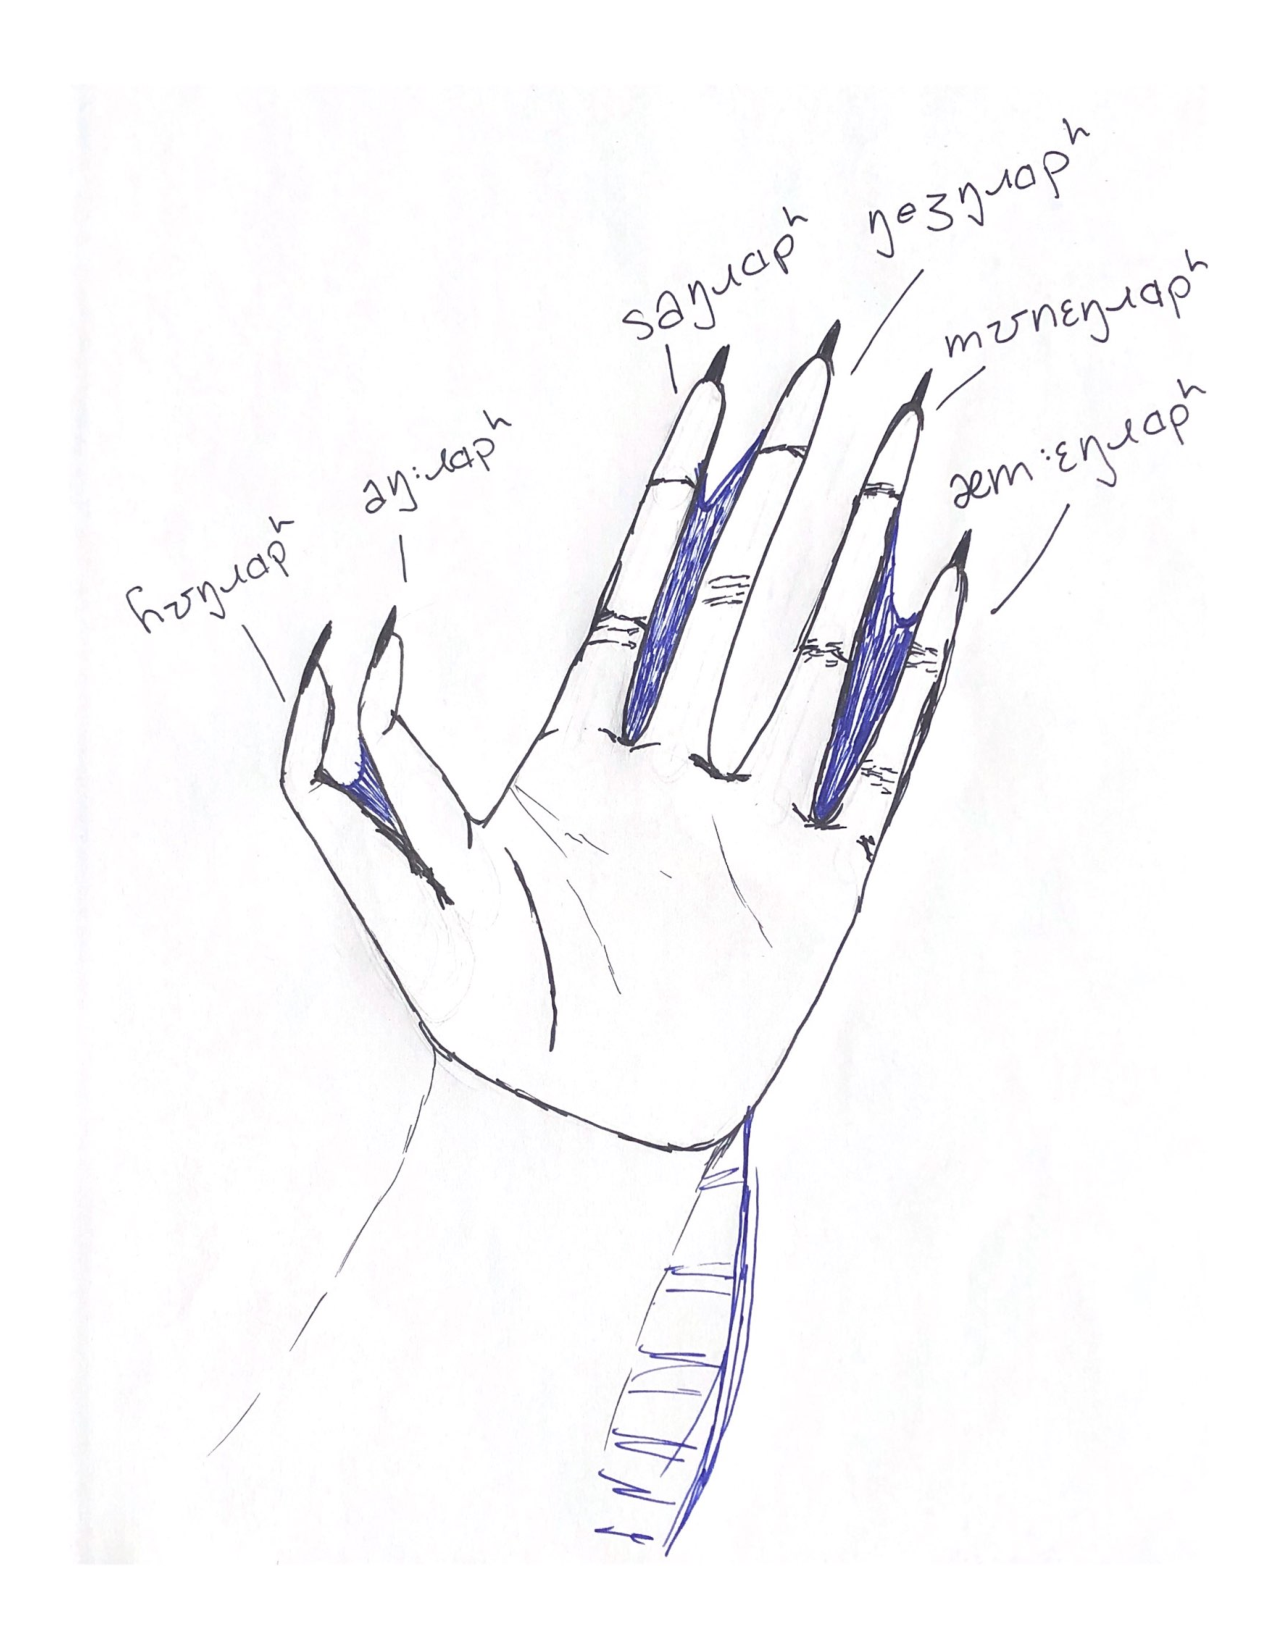
\includegraphics[scale=.7]{hand_doc.pdf}
\end{center}

\end{document}
